\documentclass{article}
\usepackage[utf8]{inputenc}
\usepackage[T1]{fontenc}
\usepackage{float}
\usepackage[table,xcdraw]{xcolor}
\usepackage{chronology}
\usepackage{graphicx}
\graphicspath{{images/}}
\usepackage{moreverb}
\usepackage{geometry}
\usepackage{array}
\usepackage{booktabs}
\usepackage{multirow}
\usepackage{url}
\usepackage[hidelinks]{hyperref}
% allow long paths/identifiers set in \texttt to break across lines
\renewcommand{\UrlFont}{\ttfamily}
\newcommand{\code}[1]{\texttt{\detokenize{#1}}}
\sloppy
 \geometry{
 a4paper,
 total={170mm,257mm},
 left=20mm,
 top=20mm,
 }

 \providecommand{\keywords}[1]
{
  \small
  \textbf{\textit{Keywords---}} #1
}

\title{Inpainting as a Data-Augmentation Method for Room-Instance Segmentation
of Architectural Floor Plans \\[1ex] \large Data Science and its Applications
project report for WiSe 2025-26}
\author{Ehsan Espandar \\ ehsan\_espandar@edu.rptu.de}
\date{10 September, 2026}

\pagenumbering{gobble}

\begin{document}

\maketitle

%TC:ignore
\begin{center}
    \begin{figure}[htbp]
      \centering
      
\includegraphics[width=0.4\textwidth]{images/rptuLogo.jpg}
    \end{figure}
    \vspace{0.8cm}

    Applied Machine Learning, Fachbereich Informatik\\

    RPTU Kaiserslautern\\
    Deutschland

    \vspace{0.8cm}

    Supervised by\\
    Darko Obradovic\\

\end{center}

\pagebreak

\pagenumbering{roman}

\begin{abstract}
Room-instance segmentation of architectural floor plans is limited by class
imbalance. In the 56-plan, 19-category dataset used here, six primary-rare room
categories contribute 70 of 1633 polygon annotations and only 17 test instances.
This report asks whether generating additional rare-room examples with diffusion
inpainting repairs that imbalance, and whether the answer depends on the
detection backbone. Fourteen augmentation arms were built from the training
split alone, covering prompt-based Stable Diffusion 1.5 inpainting, an
exemplar-guided variant with copy-paste and feather-blend controls, and a rank-8
LoRA adapter. Each arm was evaluated with a torchvision Mask R-CNN over three
seeds and with a five-fold rotated held-out cross-validation, then compared
against a fine-tuned SAM 3 and against a two-stage pipeline that labels
class-agnostic proposals with a frozen DINOv2 classifier. No diffusion or LoRA
arm produced a statistically defensible gain. On the three-seed grid the largest
class-agnostic change was $+0.036$ mask AP for plain copy-paste and $-0.057$ for
LoRA, with every paired sign test at $p \ge 0.25$, and nine of thirteen
augmented arms scored below the unaugmented baseline. Cross-validation over 21
held-out images reproduced the pattern, with copy-paste at $+0.045$ AP, positive
in all five folds at $p = 0.0625$, the minimum attainable at $K=5$. SAM 3 showed
a small multiclass gain from copy-paste, at $+0.032$, yet lost class-agnostic AP
under every augmentation, on a single seed and inside the seed-noise band
measured on the grid. Rare-class AP stayed at or near zero for every method, and
the frozen DINOv2 classifier recalled zero rare instances even on perfect
ground-truth crops. The dominant effect was the backbone. SAM 3 exceeded the
best Mask R-CNN arm by $0.089$ class-agnostic AP, an order of magnitude more
than any augmentation delta. Class-agnostic room localisation is already solved
to $0.59$--$0.71$ AP. The unsolved problem is room-type classification at this
data scale, and neither inpainting augmentation nor a dedicated frozen
classifier addressed it.
\end{abstract}

\keywords{instance segmentation; data augmentation; diffusion inpainting; LoRA;
long-tailed recognition; architectural floor plans; Mask R-CNN; SAM 3; DINOv2;
negative result}
%TC:endignore

\pagebreak

\tableofcontents
\pagebreak
\listoffigures
\pagebreak



\pagenumbering{arabic}

\setcounter{page}{1}
\section{Introduction}

Architectural floor plans encode a building as a set of labelled rooms. Turning
a scanned or exported plan back into that structured form, one polygon and one
room type per room, is an instance-segmentation problem. It is also the step
that stands between a drawing archive and any later query about areas,
circulation or fire-safety compliance. Published work on the task has
concentrated on residential plans with a handful of coarse categories
\cite{kalervo2019cubicasa5k,kratochvila2024multiunit}.

The dataset used here differs in a way that matters. It consists of German
\emph{Feuerwehrpl\"ane} (fire-brigade plans) of office and institutional
buildings, annotated with 19 functional room categories whose frequencies span
almost three orders of magnitude. Six of those categories (Allg.\
Verkehrsfl\"ache, Abstellraum, Versammlungsraum, Schacht, Garderobe,
Sanit\"arraum) account for 70 of the 1633 polygon annotations, of which 30 fall
in the training split and only 17 in the held-out test split.

That imbalance is the practical obstacle. A detector trained on the raw data
learns the frequent categories and never predicts the rare ones, so the rooms an
inspector most often needs to locate are the ones the model cannot name. The
usual remedy in the long-tailed literature is to reweight the loss or the
sampler \cite{wang2021seesaw}. A more recent remedy is to synthesise the missing
examples with a text-to-image diffusion model
\cite{xie2024mosaicfusion,shin2023fillup,wang2024doge}. Floor plans look like a
favourable setting for the synthetic route, since the drawing is mostly white
space bounded by thin black strokes. A room interior can therefore be repainted
while every wall, door, label and neighbouring room survives untouched. The
project asked one narrow question. Does diffusion or LoRA inpainting of rare
rooms improve room-instance segmentation on this dataset, and does the answer
depend on the backbone?

The work has four parts, all carried out by the author. The first is an
augmentation stack that generates rare-room examples from training-split pixels
only and admits them through automated structural and pixel checks. It produces
fourteen controlled arms covering prompt-based inpainting, an exemplar-guided
variant with copy-paste and feather-blend ablations, and a rank-8 LoRA adapter
\cite{hu2022lora} on Stable Diffusion 1.5 inpainting \cite{rombach2022ldm}. The
second part trains and evaluates every arm twice, once for the 19-class problem
and once for a derived class-agnostic view, using a torchvision Mask R-CNN
\cite{he2017maskrcnn} over three seeds. Those checkpoints were then re-evaluated
under a five-fold cross-validation that pools 21 held-out images instead of 11.
The third part carries the three most promising augmentation datasets over to a
fine-tuned SAM 3 \cite{carion2025sam3}. The fourth separates localisation from
naming: SAM 3 class-agnostic proposals are cropped and classified by a frozen
DINOv2-base encoder \cite{oquab2024dinov2}, with and without the synthetic rare
crops.

The result is negative and consistent. Across three seeds and five folds, no
diffusion or LoRA arm beat the unaugmented baseline by a margin the data
supports. Every paired sign test on the three-seed grid returned $p \ge 0.25$,
and nine of thirteen augmented arms scored below baseline on the class-agnostic
track. The only augmentation with a repeatable positive sign was plain exemplar
copy-paste, the control condition that contains no generated pixels at all. Even
its best case, $+0.045$ class-agnostic AP with all five folds positive, reaches
only $p = 0.0625$, the smallest value attainable at $K = 5$. Rare-class AP
stayed at or near zero everywhere.

What did move the numbers was the backbone. SAM 3 scored $0.713$ class-agnostic
mask AP against $0.624$ for the best Mask R-CNN arm, a gap larger than every
augmentation effect measured in the project. The two-stage experiment shows why
the negative result is still informative. Handed perfect ground-truth crops, the
frozen DINOv2 classifier recalled zero rare instances. The failure therefore
sits in room-type classification at a scale of 17 to 40 test instances. Neither
the segmentation model nor the augmentation pipeline is the limiting factor.


\section{Problem statement and Goals}

The dataset consists of 56 distinct German fire-brigade floor plans carrying
1633 polygon annotations over 19 functional room categories, partitioned by a
frozen project-aware 35/10/11 train/validation/test split in which no building
project crosses a partition boundary. The class frequencies are strongly
long-tailed. Categories 1--10 (B\"uroraum, WC, Treppe, Lager, Technikraum,
Aufzug, Andere, K\"uche, ``Flur, Halle'', Besprechungsraum) hold 1551 of the 1633
annotations. The six categories designated primary-rare --- 11 Allg.\
Verkehrsfl\"ache, 12 Abstellraum, 13 Versammlungsraum, 14 Schacht, 15 Garderobe,
16 Sanit\"arraum --- hold 70 annotations in total, of which 30 fall in the
training split and 17 in the test split. Two further categories, 17 Werkstatt
and 18 Speiseraum, are labelled low-support and reported separately; category 19
Labor has zero test instances and is excluded from every quantitative claim.
The per-split counts are given in Section~\ref{sec:dataset} and plotted in
Figure~\ref{fig:classdist}.

A detector trained on this distribution learns the head classes and assigns
essentially no probability mass to the tail, so the room types of greatest
operational interest --- shafts, storage rooms, assembly rooms --- are located but
never named, or not detected at all. The affected parties are the archive owners
who would use such a model to convert legacy plans into structured building
data, and any downstream fire-safety or facility-management query that depends on
room type rather than room geometry.

Since the drawings are line art on white ground, the interior of a single room
can be repainted by a diffusion inpainting model while every wall stroke, door
symbol, text label and neighbouring annotation is preserved exactly. This makes
the dataset an unusually clean testbed for the hypothesis that generative
augmentation can fill a long tail. The project was formulated to test that
hypothesis under conditions strict enough that a negative answer would be
informative: generation must read training-split pixels only, so that no
synthetic sample can leak validation or test information; every arm must differ
from the baseline in exactly one controlled respect; and the reported effect must
survive repetition over seeds and over evaluation splits. The problem is
therefore not ``build the best floor-plan segmenter'' but ``measure, with a
defensible error bar, whether inpainting augmentation helps, and whether that
answer is a property of the augmentation or of the backbone''.

Two evaluation views are used throughout. The \emph{multiclass} view is the
19-category instance-segmentation problem scored with COCO mask AP
\cite{lin2014coco}, plus a rare-macro AP averaged over categories 11--16 with
non-zero test support. The \emph{class-agnostic} view maps every annotation to a
single \texttt{room} category and measures whether the model finds room
boundaries at all, independent of naming. Separating the two is what allows a
change in localisation to be distinguished from a change in classification, and
it turned out to be the decisive measurement of the project.

\subsection{Goals}

\subsubsection{Goal 1: Leakage-safe augmented datasets and a controlled experiment matrix}

Build a generation stack that produces additional rare-room training examples
without ever reading a validation or test image, and wrap it in an experiment
matrix in which every arm is comparable to the unaugmented baseline. Success is
verifiable rather than statistical: every generator must be provably restricted
to the frozen training image identifiers; every accepted sample must pass
automated geometry, pixel-quality and exact-structural-invariance checks with a
recorded decision audit; every arm must use the identical model, optimiser
schedule and optimizer-step budget, and must be evaluated on the untouched test
annotations. The matrix must isolate the treatment of interest --- diffusion
inpainting --- against non-generative controls, so that a measured effect can be
attributed to the generated pixels rather than to the surrounding pipeline.

\subsubsection{Goal 2: Measure the augmentation effect on Mask R-CNN}

Quantify the effect of each augmentation arm on a torchvision Mask R-CNN, in
both the multiclass and class-agnostic views, with an error bar large enough to
support or reject a claim. This requires two independent repetitions: a grid over
three random seeds $\{42, 123, 2026\}$ for all fourteen arms, and a rotated
held-out cross-validation that re-evaluates the frozen checkpoints on five
disjoint folds of the 21 held-out images, raising the pooled rare test support
from 17 to 40 instances. Success is a statistically defensible AP delta relative
to the unaugmented arm e0 --- explicitly including the outcome that no
defensible delta exists, in which case the reported conclusion is a null result
with its $n$, standard deviation and $p$-value stated.

\subsubsection{Goal 3: Test whether a foundation-model backbone changes the verdict}

Determine whether the Mask R-CNN verdict is a property of the augmentation or of
the model class, by repeating the comparison on Meta's SAM 3 with its official
trainer, open-vocabulary text-concept head and the unchanged split. The three
most informative augmentation datasets from Goal 2 are re-used verbatim, so the
only difference between the two backbones is the backbone. Success is a direct
statement of whether the sign and magnitude of the augmentation effect are
preserved, plus a measurement of the backbone effect itself, which serves as the
scale against which every augmentation delta is judged.

\subsubsection{Goal 4: Test a two-stage DINOv2 pipeline and inpainting crops as classifier augmentation}

Separate localisation from naming by pairing a class-agnostic detector with a
frozen DINOv2-base classifier over crop features, and test whether the
inpainting-pipeline rare crops help the classifier stage where they did not help
the detector. Two evaluations are required: a ground-truth-region top-1
classification that removes detector error entirely and therefore isolates the
classification bottleneck, and an end-to-end two-stage mask AP that can be
compared directly against the fine-tuned detectors on the same test split.
Success is a diagnosis --- whether the residual error is a localisation problem
or a classification problem, and whether synthetic crops move the classification
number in either direction.


\section{Literature Review}

The reading for this project covered three strands: what is known about
augmenting instance segmentation, what is known about using generative models to
fill a long tail, and what the floor-plan and foundation-model literature offers
as backbones and datasets. Each paper below is summarised with its venue,
availability of code and data, method, main finding, and a comment on what it
implied for the design of this project.

\paragraph{Ghiasi et al., ``Simple Copy-Paste is a Strong Data Augmentation
Method for Instance Segmentation'' (CVPR 2021)
\cite{ghiasi2021copypaste}.} Code is released inside the TensorFlow TPU model
repository; the paper uses public COCO and LVIS data. The method is deliberately
minimal: instance masks are cut from one training image and pasted at random
scale and position into another, with no blending model and no attempt to make
the composite photometrically consistent. On COCO the authors report $+1.0$ box
AP over a strong baseline, and on LVIS the gain concentrates in the rare
categories ($+6.1$ mask AP for rare classes), while remaining complementary to a
long-tail loss. The finding that a crude, generator-free pixel transplant
outperforms more sophisticated composition is the single most influential result
for this project: it motivated including direct copy-paste as an explicit control
arm (e8) rather than only as an ablation, and that arm turned out to be the only
augmentation with a consistent positive sign in our own measurements.

\paragraph{Xie et al., ``MosaicFusion: Diffusion Models as Data Augmenters for
Large Vocabulary Instance Segmentation'' (IJCV 2024; arXiv:2309.13042)
\cite{xie2024mosaicfusion}.} Code and generated data are public at
\url{https://github.com/Jiahao000/MosaicFusion}. The method is training-free: an
off-the-shelf text-to-image diffusion model generates a canvas divided into
regions, each conditioned on a different category prompt, and the instance masks
are read out of the cross-attention maps rather than annotated. On LVIS the
authors report consistent gains for rare and common categories with several
detector architectures. The paper establishes the strongest form of the
hypothesis this project set out to test --- that a general-purpose diffusion
model can manufacture usable training instances for categories the detector has
barely seen. The critical difference in our setting is domain: MosaicFusion
operates on natural images, where the pretrained diffusion prior is a good model
of the data distribution, whereas a floor plan is line art the base model was
never trained to draw. Our results suggest that difference is decisive.

\paragraph{Shin et al., ``Fill-Up: Balancing Long-Tailed Data with Generative
Models'' (arXiv:2306.07200, 2023) \cite{shin2023fillup}.} Code and a project
page are available at \url{https://alex4727.github.io/Fill-Up/}. Rather than
prompting a frozen model with class names, the authors learn a textual-inversion
token per tail category from the few real examples available, then generate
synthetic images from that token until the class distribution is balanced. They
report that the inverted tokens align the synthetic images with the real domain
far better than plain prompts, and that filling the tail this way reaches
state-of-the-art results on standard long-tailed classification benchmarks when
combined with existing long-tail techniques. The paper is the direct argument for
the LoRA branch of this project: if plain prompting fails to place a class in the
right visual domain, then adapting the generator to the domain should fix it.
Our LoRA arms tested that argument on floor plans and did not reproduce the
benefit, which is worth stating precisely because the reasoning is sound and the
prior evidence is positive.

\paragraph{Wang et al., ``Domain Gap Embeddings for Generative Dataset
Augmentation'' (CVPR 2024) \cite{wang2024doge}.} Code is at
\url{https://github.com/humansensinglab/DoGE}. The method extracts the
difference between a source and a desired data distribution as a latent
embedding, then uses that embedding to steer a frozen generative model, avoiding
per-dataset fine-tuning entirely. It is evaluated under subpopulation shift and
three few-shot domain-adaptation scenarios, improving over both classical
augmentation and fine-tuned generative augmentation. The relevant lesson is
diagnostic: DoGE is built around the observation that generative augmentation
underperforms precisely when the target distribution is far from the generator's
own, which is a good description of the failure mode we observed. It also
suggests the most plausible next step for this project, since the method needs no
adapter training and would be applicable to a 30-example tail.

\paragraph{Huang et al., ``Gen-n-Val: Agentic Image Data Generation and
Validation'' (arXiv:2506.04676, 2025; CVPR 2026 Findings)
\cite{huang2025gennval}.} Code is linked from the arXiv page. The method wraps
layer-diffusion generation in an agentic loop in which a large language model
writes and revises the prompts and a vision-language model validates each
generated instance mask before it is admitted to the training set. The reported
headline is that the proportion of invalid synthetic samples drops from roughly
50\% to 7\%, with corresponding gains on rare-class instance segmentation and
open-vocabulary detection. The paper is the clearest statement in the recent
literature that the bottleneck in generative augmentation is acceptance, not
generation. Our own pipeline enforces acceptance through deterministic raster
checks --- exact invariance outside the edited region, retention of donor
strokes, pixel-statistics thresholds --- which certify structural safety but
cannot certify that the generated interior \emph{means} the requested room type.
Gen-n-Val's semantic validator is the component we lacked, and its absence is a
candidate explanation for our null result.

\paragraph{Song et al., ``TMI: Text-to-Image Meets Image-to-Image for
Complementary Data Synthesis to Boost Long-Tailed Instance Segmentation''
(arXiv:2607.08201, 2026; ECCV 2026) \cite{song2026tmi}.} Code is linked from the
arXiv page. The method combines two synthesis routes that fail differently:
text-to-image generation, which produces diverse instances but with weak
correspondence to a usable mask, and image-to-image translation of existing
annotated instances, which preserves the mask but produces little diversity. The
authors show the two are complementary on long-tailed instance-segmentation
benchmarks and that using either alone leaves most of the benefit unrealised.
This maps almost exactly onto the axis explored in our Strategy A/B (prompt-driven,
diverse, semantically unanchored) versus Strategy C (exemplar-driven,
mask-faithful, low-diversity) arms, and it predicts that neither family should
work well alone --- which is what we measured, although our experiment does not
include the combination the paper recommends.

\paragraph{Wang et al., ``Seesaw Loss for Long-Tailed Instance Segmentation''
(CVPR 2021) \cite{wang2021seesaw}.} Code is in MMDetection. Instead of adding
data, the method rebalances the classification loss with two multiplicative
factors: a mitigation factor that suppresses gradients a frequent class exerts on
a rare one, and a compensation factor that increases the penalty for
misclassifying a rare instance. It reaches a substantial rare-AP improvement on
LVIS with no change to the data pipeline. The paper is the strongest reminder
that data synthesis is not the only lever, and that a loss-side treatment is far
cheaper than a diffusion pipeline. Given our finding that the classification
stage, not the localisation stage, is the failure point, a Seesaw-style loss is
arguably the intervention this project should have tried first, and it is the
main untested alternative for future work.

\paragraph{Gupta et al., ``LVIS: A Dataset for Large Vocabulary Instance
Segmentation'' (CVPR 2019) \cite{gupta2019lvis}.} Data and evaluation code are at
\url{https://www.lvisdataset.org/}. LVIS introduced the frequent/common/rare
split protocol and the federated annotation scheme that every long-tail
instance-segmentation paper above evaluates against. It matters here mainly as a
scale reference: LVIS defines ``rare'' as fewer than 10 training images per
category across a set of 100k images, whereas our rare categories have 3--8
training instances in a set of 35 images. The methods surveyed above are
therefore validated in a regime that has two to three orders of magnitude more
data than ours, which is a caution the results section returns to.

\paragraph{Kalervo et al., ``CubiCasa5K: A Dataset and an Improved Multi-Task
Model for Floorplan Image Analysis'' (SCIA 2019)
\cite{kalervo2019cubicasa5k}.} Data and code are at
\url{https://github.com/CubiCasa/CubiCasa5k}. The paper contributes 5000
annotated Finnish residential floor plans over more than 80 object categories and
a multi-task network that predicts room segmentation, icon segmentation and wall
heatmaps from a shared encoder. It remains the standard reference dataset for
raster floor-plan parsing. Its relevance here is as a contrast: CubiCasa5K's room
classes are residential and visually distinctive, its scale is two orders of
magnitude above ours, and its plans follow a consistent drawing convention. Our
dataset shares none of those properties, which is why transferring published
architectures was never expected to be sufficient on its own.

\paragraph{Kratochvila et al., ``Recognizing and Reconstructing a Multi-Unit
Floor Plan'' (arXiv:2408.01526, 2024) \cite{kratochvila2024multiunit}.} The
paper addresses raster multi-unit plans directly, comparing U-Net variants
(MDA-UNet, MACU-Net) for pixel-wise segmentation of floor-plan structure and
reporting an F1 around 0.86 on their target elements, followed by a
vectorisation step. It is the closest recent work to our input domain, and it is
informative for two reasons. First, it confirms that structural elements ---
walls and room boundaries --- are the tractable part of the problem, which
matches our class-agnostic AP of 0.59--0.71. Second, it does not attempt
fine-grained functional room typing over a long tail, which is the part we found
to be the hard one, so it offers no evidence that the harder task is reachable at
our scale.

\paragraph{Ganon et al., ``WAFFLE: Multimodal Floorplan Understanding in the
Wild'' (arXiv:2412.00955; WACV 2025) \cite{ganon2025waffle}.} Data and code are
at \url{https://tau-vailab.github.io/WAFFLE/}. The authors assemble roughly 20k
floor plans scraped from the web, spanning building types, drawing conventions
and languages, and use large language and vision-language models to extract
semantic labels from the heterogeneous text on the drawings. They demonstrate
semantic floor-plan tasks that single-convention datasets cannot support. The
paper is the closest published example of foundation models being applied to
architectural floor plans in a few-shot manner, and it points at a resource this
project did not use: our plans carry printed German room labels
(``B\"uro'', ``Technik'') that a text-reading model could exploit directly. Given
that our vision-only classifier reached zero rare recall, reading the drawing's
own text is probably a stronger signal than anything a diffusion model can add.

\paragraph{Carion et al., ``SAM 3: Segment Anything with Concepts''
(arXiv:2511.16719, 2025) \cite{carion2025sam3}.} Code and weights are at
\url{https://github.com/facebookresearch/sam3}, gated on Hugging Face. SAM 3
extends promptable segmentation to \emph{concept} prompts: a short noun phrase
retrieves and segments all matching instances in an image, backed by a detector
with a presence head that decouples ``is this concept present'' from ``where is
it''. The model and its official trainer are the reason Goal 3 was feasible at
all --- fine-tuning it on 35 images with 19 German category names as text
concepts required a configuration change rather than a new architecture. In our
experiments it delivered the single largest effect measured in the project, which
reframed the augmentation question as a second-order one.

\paragraph{Oquab et al., ``DINOv2: Learning Robust Visual Features without
Supervision'' (TMLR 2024; arXiv:2304.07193) \cite{oquab2024dinov2}.} Code and
weights are at \url{https://github.com/facebookresearch/dinov2}. The paper
trains ViT backbones by self-distillation on a curated 142M-image corpus and
shows that the resulting frozen features support linear-probe classification,
depth estimation and segmentation at a level previously requiring supervised
fine-tuning. The practical claim exploited in Goal 4 is that a linear head on
frozen features is competitive when labelled data is scarce, which is exactly our
regime. The pretraining corpus is natural images, however, and our result ---
0.45 top-1 over 19 classes and zero recall on all six rare classes --- suggests
the frozen features do not separate functional room types in line-art drawings.

\paragraph{Zhuo et al., ``UINO-FSS: Unifying Representation Learning and
Few-Shot Segmentation via Hierarchical Distillation and Mamba-HyperCorrelation''
(arXiv:2504.15669, 2025) \cite{zhuo2025uinofss}.} The authors observe that
early-stage DINOv2 features are distributionally consistent with SAM's output
embeddings, and exploit this to distil a single backbone that serves both
representation learning and few-shot segmentation, reporting mIoU gains of
3.8--4.1 points on standard few-shot benchmarks. The paper is the strongest
recent evidence that a frozen DINOv2 encoder is a viable few-shot segmentation
substrate, and it is the reason we tested a frozen encoder rather than
fine-tuning one. Its benchmarks (PASCAL-$5^i$, COCO-$20^i$) use natural-image
classes with clear appearance signatures, which the negative outcome of our
Goal 4 experiment suggests is a load-bearing assumption.

\paragraph{Rombach et al., ``High-Resolution Image Synthesis with Latent
Diffusion Models'' (CVPR 2022) \cite{rombach2022ldm}.} Code is at
\url{https://github.com/CompVis/latent-diffusion} and the derived Stable
Diffusion 1.5 inpainting checkpoint is on Hugging Face. Running the diffusion
process in the latent space of a pretrained autoencoder rather than in pixel
space makes high-resolution synthesis and inpainting tractable on a single GPU,
and the inpainting variant conditions the denoiser on a mask and the masked
image through a nine-channel input. This is the generator used by every
diffusion arm in this project. The paper's own inpainting demonstrations are
photographic, and the qualitative failures we observed --- perspective furniture
and photographic texture rendered inside a 2D line drawing, visible in
Figures~\ref{fig:qastrategya} and \ref{fig:loraval} --- are consistent with a
prior that has essentially no floor-plan mass.

\paragraph{Hu et al., ``LoRA: Low-Rank Adaptation of Large Language Models''
(ICLR 2022) \cite{hu2022lora}.} Code is at
\url{https://github.com/microsoft/LoRA}. The method freezes the pretrained
weights and learns a low-rank update $BA$ for selected projection matrices,
reducing trainable parameters by orders of magnitude while matching full
fine-tuning quality, and adding no inference latency once merged. It has become
the standard way to adapt a diffusion U-Net to a new visual domain on a small
dataset, which is precisely what the LoRA branch of this project attempted with
rank 8 on the attention projections. The technique itself worked as advertised ---
training converged and the adapter demonstrably changed the generated
output --- but Section~\ref{sec:results} shows the adapted generator did not
produce more useful training data, and on the class-agnostic track it produced
the single worst arm in the grid.


\section{Implementation and Evaluation Details}

The project ran in four phases. Phase 1 audited and de-duplicated the source
COCO data and froze a project-aware split. Phase 2 built the generation stack and
the augmented datasets. Phase 3 ran the controlled Mask R-CNN matrix and, after
the first single-seed pass proved uninformative, extended it to three seeds and
then to a rotated held-out cross-validation. Phase 4 tested whether the verdict
was backbone-dependent, first by fine-tuning SAM 3 and then by decomposing the
task into a class-agnostic detector plus a frozen DINOv2 classifier. The
ordering was not planned in advance; each phase was a response to what the
previous one failed to show.

\subsection{Insights derived from previous work}

Three readings of the prior literature shaped the design. First, Ghiasi et al.\
\cite{ghiasi2021copypaste} report that a crude pixel transplant with no
generative model beats more elaborate composition schemes. That result made a
non-generative control mandatory: without a copy-paste arm, any gain from
diffusion inpainting could equally be a gain from ``a rare polygon appears in a
new geometric context'', which has nothing to do with the generator. The
experiment matrix was therefore structured so that the diffusion treatment is
always flanked by a copy-paste control (identical pairing, identical target
polygon, zero generated pixels) and a deterministic feather-blend control
(identical pairing, seam smoothing but no diffusion).

Second, Fill-Up \cite{shin2023fillup} and DoGE \cite{wang2024doge} both
diagnose the same failure mode --- a frozen text-to-image model asked for an
out-of-distribution class produces images that do not lie in the target domain
--- and propose opposite fixes: adapt the generator (Fill-Up, via textual
inversion) or steer the frozen generator with a domain-gap embedding (DoGE). The
LoRA branch of this project implements the first of these on Stable Diffusion 1.5
inpainting \cite{rombach2022ldm,hu2022lora}. A preliminary qualitative check
confirmed the diagnosis was applicable: prompting the pretrained model with
``architectural technical floor plan, Versammlungsraum, 2D line drawing''
produced perspective furniture and photographic texture inside the masked room
rather than 2D symbols, visible in the right-hand panels of
Figure~\ref{fig:qastrategya} and Figure~\ref{fig:loraval}.

Third, and decisively, the literature evaluates these methods in a regime with
two to three orders of magnitude more data. LVIS \cite{gupta2019lvis} defines a
rare category as one appearing in fewer than 10 of about 100k training images;
our rare categories appear 3--8 times in a 35-image training split, and are tested
on 1--6 instances each. This is what motivated the class-agnostic track and,
later, the cross-validation and the two-stage decomposition: if a null result
was going to be reported, it had to be accompanied by evidence about
\emph{why} it was null, and about whether the measurement itself was capable of
detecting an effect.

\subsection{Technologies used}

Table~\ref{tab:tech} lists the main components. PyTorch and torchvision were
chosen for the detector because \protect\path{maskrcnn_resnet50_fpn_v2} provides a
well-understood, pretrained instance-segmentation baseline that trains on a
single GPU with a 35-image training set --- the point of the baseline is that it
is unremarkable, so that any measured difference is attributable to the data.
Hugging Face \texttt{diffusers} supplies the Stable Diffusion 1.5 inpainting
pipeline, whose nine-channel mask conditioning is what makes bit-exact
preservation outside the edited region possible. \texttt{peft} provides the LoRA
implementation. SAM 3 was run through Meta's own training harness rather than a
reimplementation, so that the comparison is against the model as its authors
configured it. DINOv2-base was loaded through \texttt{transformers} and used
strictly as a frozen feature extractor. Shapely handles polygon clipping when
crops are cut out of a plan, and \texttt{pycocotools} computes every AP reported
in this report, so that all numbers use the standard COCO definition
\cite{lin2014coco}.

\begin{table}[H]
\centering
\caption{Main technologies and their role in the project.}
\label{tab:tech}
\footnotesize
\begin{tabular}{@{}p{0.26\textwidth}p{0.30\textwidth}p{0.36\textwidth}@{}}
\toprule
Component & Version / identifier & Role \\
\midrule
PyTorch + torchvision & 2.1.2 (env \texttt{inpainting}) & Mask R-CNN training and evaluation \\
Mask R-CNN & \protect\path{maskrcnn_resnet50_fpn_v2}, ImageNet & baseline detector, both tracks \\
Stable Diffusion 1.5 inpainting & rev.\ \texttt{8a4288a7} & Strategy A/B/C generators \\
\texttt{diffusers}, \texttt{peft} & pinned in \texttt{requirements.txt} & diffusion pipeline, rank-8 LoRA \\
SAM 3 & \protect\path{facebookresearch/sam3} (env \texttt{sam3}, torch 2.10) & foundation-model detector \\
DINOv2-base & \texttt{facebook/dinov2-base} & frozen crop encoder, stage 2 \\
\texttt{pycocotools} & --- & COCO bbox/mask AP for every result \\
Shapely & --- & polygon clipping for rare-centred crops \\
Slurm & DFKI Pegasus cluster, A100/H100 & job orchestration \\
\bottomrule
\end{tabular}
\end{table}

\subsection{Student's contribution}

The pretrained weights (ImageNet, Stable Diffusion 1.5 inpainting, SAM 3,
DINOv2-base), the SAM 3 training harness, and the source COCO annotation file
are existing work. Everything else in the repository was designed and
implemented by the author: the Phase-1 audit and SHA-256 de-duplication; the
seeded project-aware split search; the safe-mask construction that erodes a room
polygon, subtracts overlapping annotations and protects detected dark strokes;
all three generation strategies and the LoRA training and conversion scripts;
the automated quality-control rules and the immutable decision audit; the
experiment runner with its fixed optimizer-step budget and provenance check that
rejects any augmented image not traceable to a training-split identifier; the
bounded rare-aware sampler; the class-agnostic dataset view; the SAM 3
configuration and the two bug fixes described in
Section~\ref{sec:problems}; the rotated held-out cross-validation; the DINOv2
feature extraction and two-stage evaluation; and the analysis scripts that
produce every table and figure in this report. The interpretation, the
statistical protocol and the decision to report a null result are likewise the
author's.

\subsection{Dataset Description and preprocessing}
\label{sec:dataset}

The source is a COCO-format collection of German fire-brigade floor plans
(\protect\path{area_segmentation_coco}) with 60 images, 1709 polygon annotations and
19 room categories. A Phase-1 audit verified that every referenced image file
exists and that every annotation is a valid polygon. SHA-256 comparison of the
image bytes identified four exact duplicates (COCO image IDs 22, 24, 25 and 26),
which were removed from the annotation file; the source JPEGs were left
untouched. The working dataset is therefore 56 images with 1633 annotations
over 19 categories, with model labels $1\ldots19$ and background $0$.

The plans come from 12 distinct building projects, and several plans of the same
project are near-identical floors of the same building. A random image-level
split would therefore place near-duplicates of the same floor on both sides of
the split. The split was instead generated by a seeded search over project-level
assignments, subject to the constraint that no project may contribute images to
more than one partition, and scored on how well it preserved rare-class coverage
in the test partition. The resulting frozen split assigns 35 images to train
(projects P01, P03, P05, P06, P08, P10--P13), 10 to validation (P02) and 11 to
test (P04, P07). It deviates from a 70/15/15 target in favour of valid rare-class
test coverage, which was judged the more useful property.

\begin{table}[H]
\centering
\caption{Per-class instance counts in the frozen project-aware split.
Categories 11--16 are the primary-rare group, 17--18 are low-support, and
category 19 has zero test instances and is excluded from all quantitative
claims. Source: \protect\path{outputs/splits/class_distribution_by_split.csv}.}
\label{tab:classdist}
\small
\begin{tabular}{@{}rlrrrr@{}}
\toprule
ID & Category & Train & Val & Test & Total \\
\midrule
1  & B\"uroraum            & 155 & 117 & 102 & 374 \\
2  & WC                    & 170 & 53  & 33  & 256 \\
3  & Treppe                & 117 & 38  & 57  & 212 \\
4  & Lager                 & 87  & 44  & 55  & 186 \\
5  & Technikraum           & 113 & 29  & 36  & 178 \\
6  & Aufzug                & 128 & 1   & 13  & 142 \\
7  & Andere                & 38  & 18  & 22  & 78  \\
8  & K\"uche               & 17  & 16  & 16  & 49  \\
9  & Flur, Halle           & 8   & 30  & 3   & 41  \\
10 & Besprechungsraum      & 16  & 8   & 11  & 35  \\
\midrule
11 & Allg.\ Verkehrsfl\"ache & 3 & 12  & 1   & 16  \\
12 & Abstellraum           & 8   & 1   & 2   & 11  \\
13 & Versammlungsraum      & 8   & 0   & 5   & 13  \\
14 & Schacht               & 3   & 7   & 2   & 12  \\
15 & Garderobe             & 4   & 0   & 6   & 10  \\
16 & Sanit\"arraum         & 4   & 3   & 1   & 8   \\
\multicolumn{2}{@{}l}{\emph{primary-rare subtotal}} & 30 & 23 & \textbf{17} & 70 \\
\midrule
17 & Werkstatt             & 4   & 0   & 1   & 5   \\
18 & Speiseraum            & 1   & 1   & 2   & 4   \\
19 & Labor                 & 3   & 0   & 0   & 3   \\
\midrule
\multicolumn{2}{@{}l}{\textbf{All categories}} & \textbf{887} & \textbf{378} & \textbf{368} & \textbf{1633} \\
\bottomrule
\end{tabular}
\end{table}

Figure~\ref{fig:classdist} shows the same distribution graphically and
Figure~\ref{fig:raresupport} isolates the tail. The consequence that governs the
whole report is in the ``Test'' column: the six primary-rare categories are
scored on 17 instances in total, and three of them on two instances or fewer. A
COCO AP computed over one or two instances is a step function; it cannot express
a small improvement.

\begin{figure}[H]
\centering
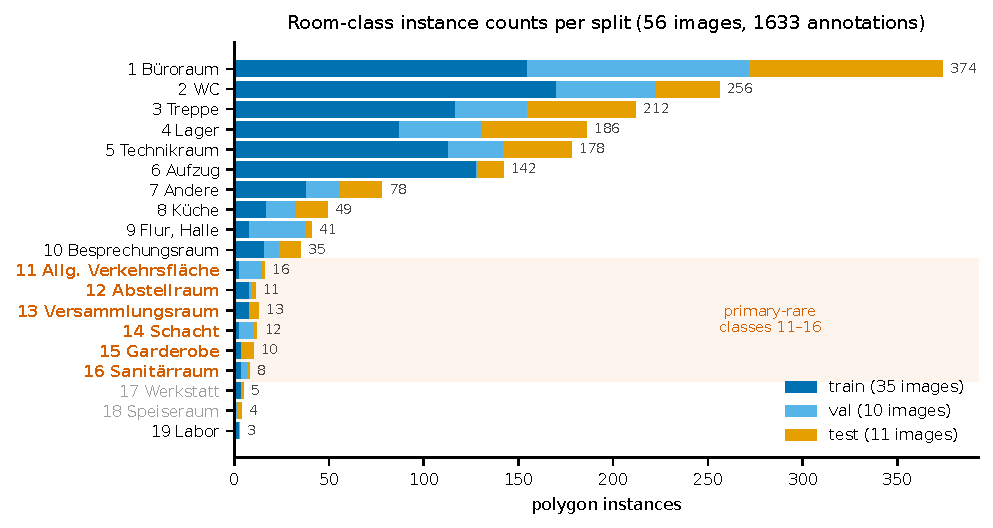
\includegraphics[width=\textwidth]{images/fig_class_distribution.pdf}
\caption{Room-class instance counts per split.}
\label{fig:classdist}
\end{figure}

\begin{figure}[H]
\centering
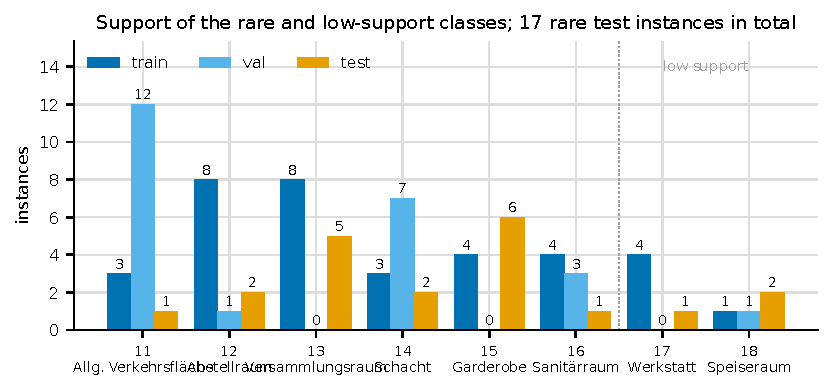
\includegraphics[width=\textwidth]{images/fig_rare_support.pdf}
\caption{Support of the rare and low-support classes.}
\label{fig:raresupport}
\end{figure}

A second view of the same data was derived for the class-agnostic track. It
preserves all 56 image records, all 1633 annotation identifiers, polygons,
bounding boxes and areas, and the frozen split, and rewrites every category to a
single foreground class \texttt{room}. The detector then has two classes instead
of twenty. Because the two views differ only in the label field, a difference
between the tracks is a difference between ``finding rooms'' and ``naming
rooms''.

\subsubsection*{Generation strategies}

All generators read the frozen training image identifiers and nothing else; the
loader traces every augmented image back to a training identifier and rejects
validation or test provenance rather than silently filtering. Three strategies
were implemented.

\emph{Strategy A} converts a real rare room into a different appearance of the
same rare class. The room polygon is rasterised at original resolution, eroded
by $\mathrm{round}(\mathrm{clamp}(0.02\cdot\min(w,h),2,12))$ pixels to protect
its walls, intersected against all overlapping annotations, and dark strokes
detected by Otsu thresholding inside the room are dilated by two pixels and
protected. Only the resulting safe mask is editable. A crop with one bounding-box
width and height of context on each side is white-padded and resized to $512^2$,
inpainted, inverse-mapped, and composited back through the original-resolution
safe mask. The written PNG is reopened and compared against the source: exact
invariance outside the safe mask is mandatory and cannot be disabled by
configuration. Figure~\ref{fig:qastrategya} shows the seven-panel audit row
produced for every candidate.

\emph{Strategy B} converts a \emph{common} room into a rare one. Common classes
1--10 are screened against the real rare-class ranges of area, aspect ratio,
width, height and polygon solidity (5th--95th percentile expanded by 50\%), each
source annotation is used at most once, and the per-class target is
$\min(3 \times n_{\mathrm{real}}, 20)$. Only the selected annotation's category
label changes; its polygon and every other annotation stay as they are.

\emph{Strategy C} is exemplar-guided. Instead of asking the model to invent a
rare room, a real rare training room is transplanted into a geometry-compatible
common-room polygon: both polygons are rasterised, the target interior is
cleared, the donor bounding box and mask are affinely mapped onto the target, and
only donor pixels are inserted. Diffusion is then restricted to a narrow inner
seam and to editable target pixels the warped donor does not cover, at strength
0.30 --- the core donor pixels lie outside the diffusion mask by construction.
Three modes were generated from the identical pairing plan so that the diffusion
contribution is isolated: C0 direct copy-paste (no generated pixels, arm e8), C1
deterministic feather blending (arm e9), and C2 exemplar-seeded diffusion
inpainting (arms e10/e11). Figure~\ref{fig:qastrategyc} shows a C0 audit row.

\emph{The LoRA branch} trains one shared rank-8 adapter on the attention
projections of the SD 1.5 inpainting U-Net, freezing the VAE, text encoder and
base U-Net. Training crops are room-centred $512^2$ crops from training
annotations only, with 12 deterministic classical variants per usable rare crop
(brightness, contrast, grayscale, mild blur, scan noise, line-thickness and a
small geometry-aligned affine); those variants share a
\protect\path{source_annotation_id} and are explicitly recorded as \emph{not}
independent geometries. The prompt template is ``architectural technical floor
plan, \{category\_name\}, 2D line drawing''. The trained adapter then drives a
Strategy-B-style common-to-rare conversion (arms e12/e13).
Figure~\ref{fig:loraval} is the fixed-seed validation contact sheet comparing
pretrained SD against the adapter on the same source, mask and seed.

Acceptance is fully automatic and auditable. A candidate is rejected for an
empty or too-small editable region, a near-identical or blank or uniform output,
an extreme increase in dark or saturated fill, a safety-checker flag, any changed
pixel outside the editable interior or on the protected boundary, or a hash
mismatch on the written file. Table~\ref{tab:acceptance} reports the outcome.
These are raster checks only: they certify that the surrounding drawing is
untouched and that the edited region is not degenerate, but they cannot certify
that the generated interior depicts the requested room type. Every strategy's
metadata therefore records \protect\path{semantic_correctness = unverified}, except
Strategy C, which records \protect\path{real_train_exemplar_preserved} because its
rare pixels are copied from a real annotated room of that class.

\begin{table}[H]
\centering
\caption{Automated acceptance of generated candidates, per generation branch.
Sources: \protect\path{outputs/augmentation_a/summary.json},
\protect\path{augmentation_b/summary.json}, \protect\path{augmentation_c/*/summary.json},
\protect\path{augmentation_lora_b/summary.json}. ``Rare geometries added'' counts
common-room polygons relabelled to a rare class; for Strategy A the edit changes
the appearance of an existing rare room, so no new rare polygon is created.}
\label{tab:acceptance}
\small
\begin{tabular}{@{}llrrrl@{}}
\toprule
Branch & Arms & Attempted & Accepted & Rate & Dominant rejection reasons \\
\midrule
A (prompt, rare$\rightarrow$rare)   & e2--e5   & 90 & 74 & 0.82 & extreme dark filling (14) \\
B (prompt, common$\rightarrow$rare) & e6--e7   & 40 & 27 & 0.68 & safe mask too small (8) \\
C0 copy-paste                       & e8       & 52 & 46 & 0.88 & editable region too small (5) \\
C1 feather blend                    & e9       & 52 & 45 & 0.87 & editable region too small (5) \\
C2 diffusion inpaint                & e10--e11 & 52 & 45 & 0.87 & editable region too small (5) \\
LoRA (prompt, common$\rightarrow$rare) & e12--e13 & 52 & 31 & 0.60 & generated region uniform (10) \\
\bottomrule
\end{tabular}
\end{table}

\begin{figure}[H]
\centering
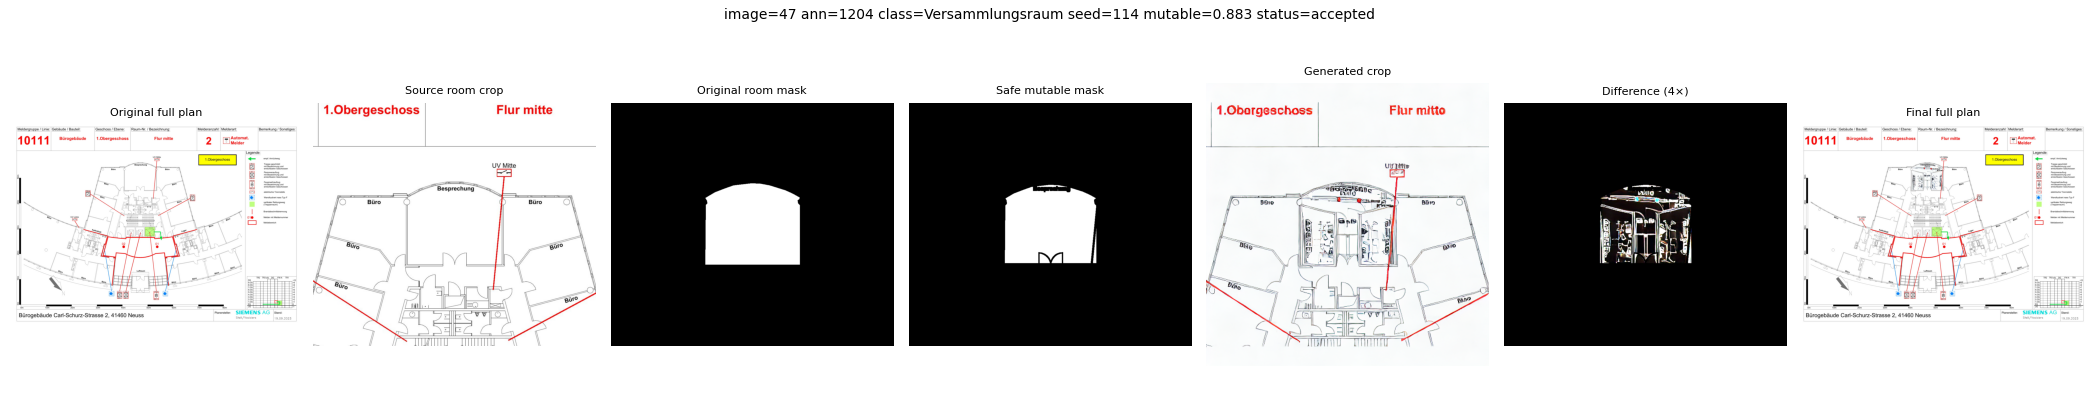
\includegraphics[width=\textwidth]{images/strategy_a_row.png}
\caption{Strategy A quality-control audit row (accepted candidate).}
\label{fig:qastrategya}
\end{figure}

The Strategy A row in Figure~\ref{fig:qastrategya} is worth reading closely,
because it shows both that the safety machinery works and that the semantics do
not. The ``Difference'' panel is confined entirely to the safe mask, so the
surrounding plan is bit-identical --- but the ``Generated crop'' contains
perspective furniture and photographic shading, not the 2D symbols of a German
Versammlungsraum. This candidate passed every automated check and entered the
training set.

\begin{figure}[H]
\centering
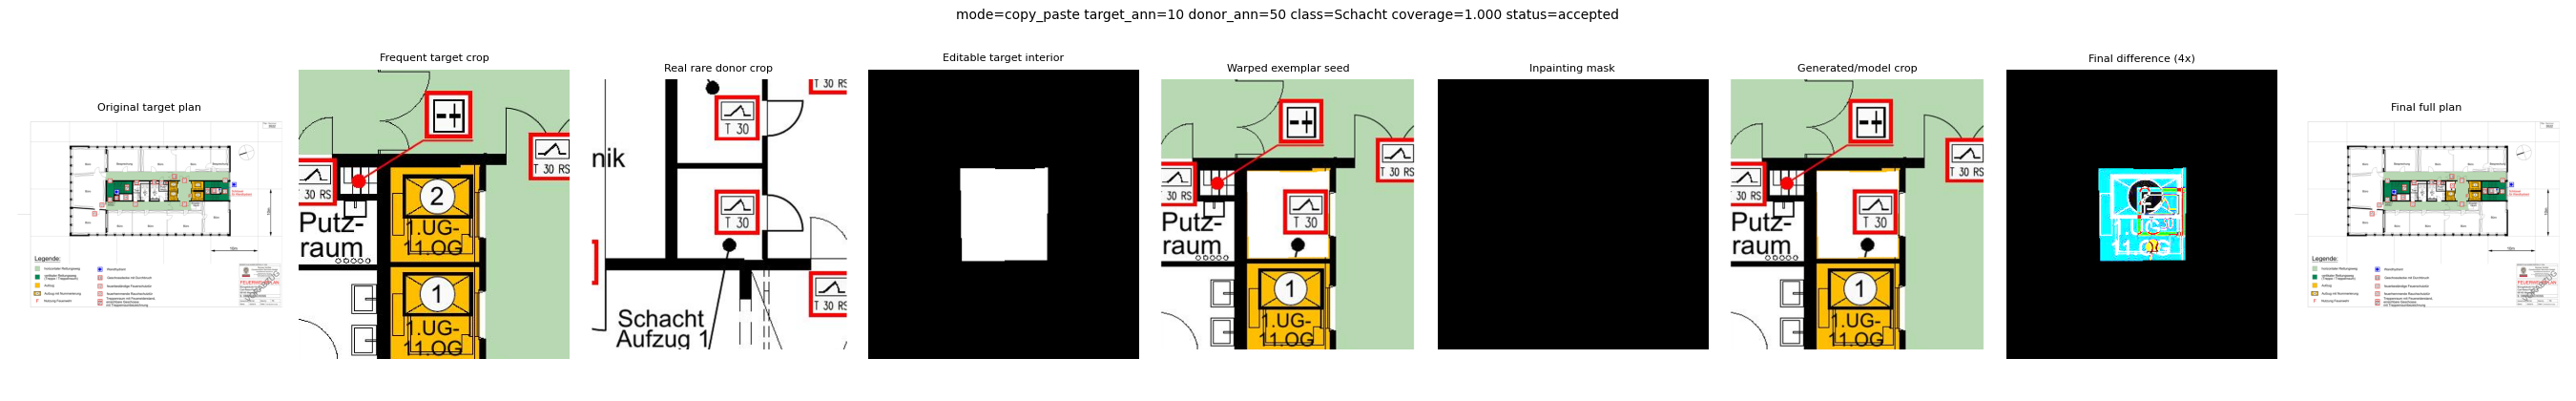
\includegraphics[width=\textwidth]{images/strategy_c_copypaste_row.png}
\caption{Strategy C exemplar copy-paste audit row.}
\label{fig:qastrategyc}
\end{figure}

\begin{figure}[H]
\centering
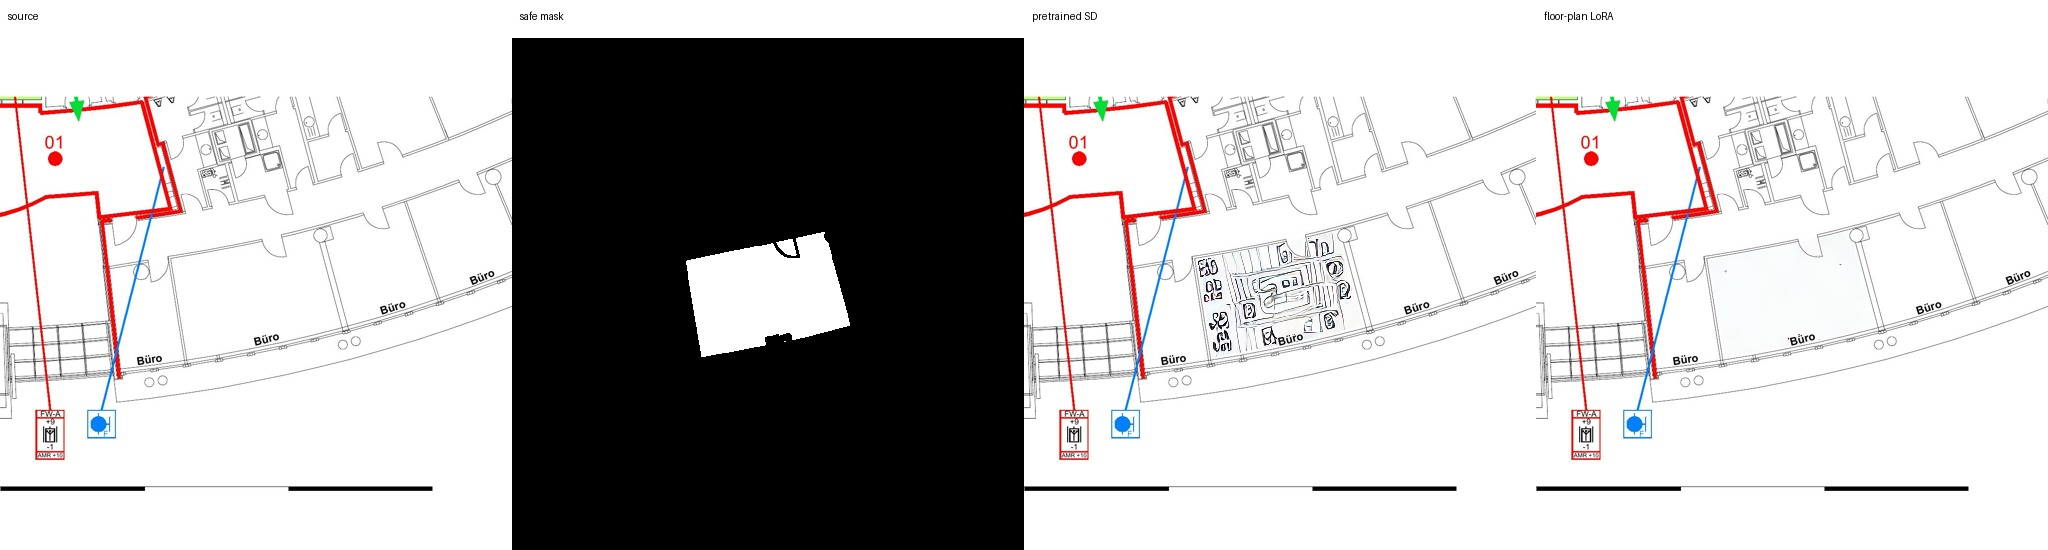
\includegraphics[width=\textwidth]{images/lora_val_13.jpg}
\caption{Pretrained Stable Diffusion versus the floor-plan LoRA on a fixed case.}
\label{fig:loraval}
\end{figure}

Figure~\ref{fig:loraval} isolates what the adapter learned. Given the same
source, safe mask and seed, pretrained SD (third panel) fills the room with
dense pseudo-furniture, while the LoRA (fourth panel) produces a nearly empty
light-grey region. The adapter successfully learned that floor plans are mostly
white space --- and, because the mask construction protects detectable dark
strokes, it was largely trained on regions from which the strongest category cues
had already been removed. The result is safe and domain-consistent output that
carries no room-type information, which is a plausible mechanism for the
downstream measurements in Section~\ref{sec:results}.

\subsection{Experimental Setup and Evaluation}

Every experiment reports COCO bbox and mask AP computed by \texttt{pycocotools}
against the untouched test annotations \cite{lin2014coco}. The multiclass track
additionally reports a rare-macro mask AP, defined as the unweighted mean over
categories 11--16 that have non-zero test support. The class-agnostic track
reports overall \texttt{room} AP; rare-macro AP is undefined there. Augmented
data is used for training only; validation and test always use the original
held-out images and annotations.

\subsubsection{Goal 1: the controlled experiment matrix}

Fourteen arms were defined, listed in Table~\ref{tab:arms}. Each arm declares
both tracks, and each is trained from independent ImageNet initialisation with
the identical recipe: \protect\path{maskrcnn_resnet50_fpn_v2}, 25 epochs, exactly 35
optimizer steps per epoch, SGD at learning rate 0.005 with momentum 0.9 and
weight decay $5\times10^{-4}$, a step schedule dropping by $0.1$ every 8 epochs,
batch size 1, aspect-preserving resize with \texttt{min\_size} 1024 and
\texttt{max\_size} 1600, AMP, and horizontal flip plus mild photometric jitter.
Fixing the optimizer-step budget rather than the epoch count over a larger
dataset is what makes the arms comparable: an augmented arm sees a different
\emph{mixture} of images than e0, but not more gradient updates. The best
checkpoint is selected on validation mask AP.

The rare-aware sampler used by the ``$+$w'' arms assigns each training image the
bounded weight
\[
  w_i \;=\; \min\!\left(5,\; 1 + 2\sum_c \frac{n_{ic}}{\sqrt{n^{\mathrm{real}}_c}}\right),
\]
where $n_{ic}$ counts instances of class $c$ in image $i$ and
$n^{\mathrm{real}}_c$ is the class count in the \emph{original} training
annotations, so that synthetic images cannot inflate their own weight. The cap
bounds any single image's sampling probability.

\begin{table}[H]
\centering
\caption{The fourteen controlled arms. ``$+$w'' denotes bounded rare-aware image
sampling; ``$+$crop'' mixes rare-centred crops with full plans at probability
$0.4/0.6$. Every arm runs both the multiclass and the class-agnostic track.}
\label{tab:arms}
\small
\begin{tabular}{@{}llll@{}}
\toprule
Arm & Training data & Sampling & Role \\
\midrule
e0  & original 35 plans                & uniform & baseline \\
e1  & original 35 plans                & rare-weighted & sampling-only control \\
e2  & $+$ Strategy A                   & uniform & prompt inpainting, rare$\rightarrow$rare \\
e3  & $+$ Strategy A                   & rare-weighted & A $\times$ sampling \\
e4  & $+$ Strategy A $+$ crops         & uniform & A $\times$ crop mixing \\
e5  & $+$ Strategy A $+$ crops         & rare-weighted & A $\times$ crops $\times$ sampling \\
e6  & $+$ Strategy B                   & uniform & prompt inpainting, common$\rightarrow$rare \\
e7  & $+$ Strategy B                   & rare-weighted & B $\times$ sampling \\
e8  & $+$ Strategy C0 copy-paste       & uniform & \emph{non-generative control} \\
e9  & $+$ Strategy C1 feather blend    & uniform & deterministic-blending control \\
e10 & $+$ Strategy C2 diffusion inpaint& uniform & \emph{primary inpainting treatment} \\
e11 & $+$ Strategy C2 diffusion inpaint& rare-weighted & C2 $\times$ sampling \\
e12 & $+$ LoRA Strategy B              & uniform & adapted-generator treatment \\
e13 & $+$ LoRA Strategy B              & rare-weighted & LoRA $\times$ sampling \\
\bottomrule
\end{tabular}
\end{table}

Goal 1 is verified rather than scored: all generators were confirmed to read only
frozen training identifiers, every accepted sample carries a recorded
quality-control decision and output hash, and every arm ran both tracks under the
identical budget. Table~\ref{tab:acceptance} is the corresponding evidence.

\subsubsection{Goal 2: the three-seed grid and the rotated held-out cross-validation}

The grid runs all 14 arms $\times$ 2 tracks $\times$ 3 seeds $\{42, 123, 2026\}$,
for 84 training runs. Per-arm results are the mean and population standard
deviation over the three seeds. Each augmented arm is compared to e0 by a paired
test over the seeds --- Wilcoxon signed-rank where applicable, falling back to an
exact two-sided sign test. At $n=3$ the smallest attainable two-sided sign-test
$p$-value is $0.25$, which occurs only when all three seed-level differences share
a sign; this ceiling is a property of the design and is stated with every
$p$-value in Section~\ref{sec:results}.

The single-seed pass that preceded the grid produced apparently large effects
(for example, Strategy A at $0.121$ multiclass mask AP against $0.075$ for e0 on
seed 42 alone) that did not survive the addition of two further seeds. That
experience is why no single-seed number is treated as evidence anywhere in this
report.

The grid's weakness is the 11-image test split. The rotated held-out
cross-validation addresses it without retraining anything. The 35-image training
split is held fixed for every fold --- so the augmented datasets, which are built
from that split, and all grid checkpoints remain valid --- and only the
evaluation set rotates: the 21 held-out images (validation $+$ test) are
partitioned round-robin into $K=5$ folds, and each frozen checkpoint is
re-evaluated on each fold in evaluation-only mode. Across the folds every
held-out image is tested exactly once, and the pooled rare test support rises
from 17 to 40 instances. Six arms $\{$e0, e1, e6, e8, e10, e12$\}$ were selected
to span the families, giving $6 \times 2 \times 5 = 60$ evaluations. The
project-aware constraint is not violated: the 21 held-out images span only three
projects, so a project-aware $K>3$ partition is impossible, but the only leakage
that could matter --- between the frozen training split and the evaluation images
--- is prevented by construction because no fold trains anything. Per-fold
paired tests against e0 use the same sign-test protocol; at $K=5$ the minimum
attainable two-sided $p$-value is $0.0625$.

\subsubsection{Goal 3: SAM 3}

SAM 3 \cite{carion2025sam3} was fine-tuned with Meta's official trainer on the
unchanged split, using the 19 German category names as text concepts for the
multiclass track and a single \texttt{room} concept for the class-agnostic track.
The configuration is 20 epochs at resolution 1008, AdamW with gradient clipping
at max-norm 0.1, layer-wise learning-rate decay of 0.9 on the vision trunk, and
three learning-rate groups on an inverse-square-root schedule --- $8\times10^{-5}$
for the heads, $2.5\times10^{-5}$ for the vision backbone and $5\times10^{-6}$
for the language backbone --- with instance-mask loss and the model's presence
head enabled at evaluation. Evaluation writes COCO prediction JSON and is scored
with the same \texttt{pycocotools} path as the Mask R-CNN runs, so the two
backbones' numbers are directly comparable.

Three augmentation datasets were carried across verbatim, without regeneration:
Strategy C2 diffusion inpaint (the e10 data), LoRA Strategy B (the e12 data) and
Strategy C0 copy-paste (the e8 data). Each was run once per track, giving a
baseline plus three augmented runs in each of the two tracks. These are
single-seed runs; the seed-to-seed standard deviation measured on the grid is the
noise floor against which their deltas must be read, and Section~\ref{sec:results}
does exactly that.

\subsubsection{Goal 4: the two-stage DINOv2 pipeline}

The two-stage pipeline is drawn in Figure~\ref{fig:pipeline}. Stage 1 is the
already-trained class-agnostic SAM 3 detector, which contributes 483 test
proposals. Each proposal or annotation bounding box is expanded by a context
margin, clamped to the image, padded to a white square and resized to $224^2$.
Stage 2 encodes the crop with a frozen DINOv2-base \cite{oquab2024dinov2} and
represents it by the concatenation of the CLS token and the mean of the patch
tokens, a 1536-dimensional vector; features are standardised and
$\ell_2$-normalised. Two heads were trained on those features: a linear
classifier (Adam, 300 epochs, inverse-square-root class weighting) and a cosine
$k$-NN with $k=5$. No gradient reaches the backbone in either case.

\begin{figure}[H]
\centering
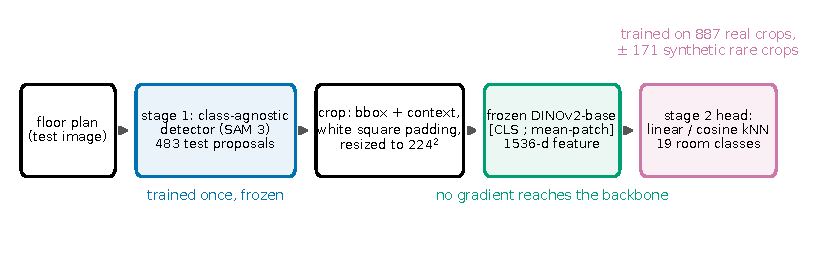
\includegraphics[width=\textwidth]{images/fig_twostage_pipeline.pdf}
\caption{The two-stage room-typing pipeline.}
\label{fig:pipeline}
\end{figure}

Two arms differ only in the head's training set: \texttt{real} uses the 887 real
training-split ground-truth crops, and \texttt{real\_plus\_synth} adds the 171
rare crops produced by the augmentation pipeline. Two evaluations are reported.
Evaluation A classifies the 368 real ground-truth test crops, which removes
detector error entirely and therefore measures the classification bottleneck in
isolation; it reports top-1 accuracy, head-macro recall over classes 1--10 and
rare-macro recall over 11--16. Evaluation B labels the 483 class-agnostic test
proposals with the head and scores the result as multiclass instance
segmentation with \texttt{COCOeval(segm)} against the multiclass test ground
truth, which puts the two-stage system on exactly the same axis as the
end-to-end fine-tuned detectors.

\subsection{Ethical considerations}

The dataset contains architectural drawings of real, identifiable buildings ---
specifically fire-brigade plans, which mark escape routes, hydrants and shafts.
It contains no personal data and no images of people, so the privacy exposure is
institutional rather than individual, but the plans are not public documents and
were not redistributed. All diffusion inference ran locally on cluster nodes
against a pre-downloaded model cache with Hugging Face offline mode enabled, so
no floor-plan image was transmitted to a third-party service at any point. The
Stable Diffusion safety checker was retained rather than disabled; it flagged and
rejected a small number of candidates (two in Strategy A, two in C2, two in the
LoRA branch), which were discarded like any other rejection.

The clearest ethical risk in the work is the synthetic data itself. The
generation pipeline produces images that look like genuine fire-brigade plans but
in which a room has been silently relabelled --- a Technikraum redrawn and
annotated as a Schacht. Such an image is safe as a training sample and unsafe as
a document: if it escaped the training directory it could be mistaken for a real
plan of a real building, with obvious consequences for anyone relying on it in an
emergency. The pipeline mitigates this by construction rather than by convention:
synthetic images live in separate \protect\path{data/augmented_*} directories, carry a
\texttt{strategy} field and a stable synthetic identifier in their COCO records,
and are never written back into the source dataset, which remains byte-identical
throughout. This report reproduces synthetic panels only inside labelled
quality-control figures.

A second concern is honest reporting. Generation-side metadata records
\protect\path{semantic_correctness = unverified} wherever automatic checks cannot
establish that a generated region depicts the requested class, and the file
\protect\path{outputs/augmentation_b/review.csv} is explicitly an automatic decision
audit rather than a human review gate. Related to this, the LoRA branch
documentation records that the prompt-only conversion retained visible
common-room text labels such as ``B\"uro'' in some accepted samples; the e12/e13
results are reported here as measurements of that data as it was actually used,
with the caveat stated, rather than quietly dropped. The project's central claim
is a negative one, and it is reported as such --- with $n$, standard deviation
and $p$-value --- rather than being narrowed to the subset of arms and metrics
that happen to look favourable.

\subsection{Reproducibility and code availability}

All code, configuration, tests and documentation are in a single Git repository
at commit \texttt{d1b08f0}; datasets, model weights and outputs are
machine-local and deliberately untracked. The cluster checkout lives in one
directory, \protect\path{/netscratch/espandar/inpainting/floorplan-inpainting/}, with
code in \texttt{src/}, \texttt{scripts/}, \texttt{slurm/} and \texttt{configs/},
derived datasets in \texttt{data/}, adapters in \texttt{models/} and every
result, checkpoint and log below \texttt{outputs/}. The consolidated summaries
that this report cites are in \texttt{outputs/final/}: \texttt{grid\_r1/},
\texttt{cv/}, \texttt{sam3/} and \texttt{dino/}, each holding a
\texttt{summary.json} and \texttt{summary.csv}.

Two conda environments are used because the two backbones have incompatible
requirements: \texttt{inpainting} (PyTorch 2.1.2) for data preparation, the
diffusion generators, Mask R-CNN and the DINOv2 stage, and \texttt{sam3}
(PyTorch 2.10) for SAM 3. Experiments run on the DFKI Pegasus Slurm cluster on
A100 and H100 nodes; SAM 3 jobs are pinned to the 80\,GB GPU tier. Four submit
scripts reproduce the whole set of results, each of them a dependency chain of
the form ``build inputs $\rightarrow$ smoke test one task $\rightarrow$ full array
$\rightarrow$ analyse'':

\begin{table}[H]
\centering
\caption{Reproduction entry points. Each script is run from the project
directory on the cluster and writes its consolidated result under
\texttt{outputs/final/}.}
\label{tab:repro}
\small
\begin{tabular}{@{}lll@{}}
\toprule
Script & Work & Output \\
\midrule
\protect\path{scripts/submit_grid_r1.sh}  & 14 arms $\times$ 2 tracks $\times$ 3 seeds & \protect\path{outputs/final/grid_r1/} \\
\protect\path{scripts/submit_cv.sh}        & 5-fold rotated held-out re-evaluation & \protect\path{outputs/final/cv/} \\
\protect\path{scripts/submit_sam3_aug.sh} & SAM 3 baseline $+$ 3 augmentations, 2 tracks & \protect\path{outputs/final/sam3/} \\
\protect\path{scripts/submit_dino.sh}      & DINOv2 extraction, heads and two-stage eval & \protect\path{outputs/final/dino/} \\
\bottomrule
\end{tabular}
\end{table}

Determinism is bounded and stated rather than promised. Split generation, seed
assignment, sampler construction, candidate ordering and quality-control
thresholds are fully deterministic, and every generated sample carries a stable
identifier, its seed, the exact model revision
(\texttt{8a4288a76071f7280aedbdb3253bdb9e9d5d84bb}), the LoRA weight hash and the
output file hash, so an interrupted run resumes by sample identifier and a
changed configuration is forced into a new output directory. Diffusion sampling
reproduces a given candidate on the same software and GPU stack, but bitwise
reproducibility across different GPU models is not claimed. Detector training
uses AMP and a fixed seed, and the seed-to-seed spread reported in
Section~\ref{sec:results} is precisely the residual variation this leaves.
The figures in this report are regenerated from the fetched summary files by
\protect\path{report/scripts/make_figures.py}, which is committed alongside them.

At the time of writing the repository has not been pushed to a public forge, so
the cluster checkout is synchronised in place from the local \texttt{main}
branch by \protect\path{scripts/deploy_cluster.sh}, which ships the history as a Git
bundle and fast-forwards the remote checkout. Once a hosted remote is
configured this is replaced by an ordinary \texttt{git pull} and the bundle
mechanism can be deleted. Code availability to a third party is therefore
currently by request rather than by URL.

\subsection{Problems faced during the project}
\label{sec:problems}

\emph{The test split is too small to measure the thing the project is about.}
This is the fundamental problem, and it was not solved. Six rare categories are
scored on 17 test instances, three of them on two instances or fewer. A COCO AP
over two instances takes a handful of discrete values, so a genuine small
improvement in rare-class segmentation is not representable, let alone
distinguishable from noise. Two mitigations were built --- three seeds, to
measure the noise, and the rotated cross-validation, to raise the pooled rare
support from 17 to 40 --- and both helped characterise the measurement without
removing the ceiling. The honest statement of the outcome is that the experiment
can exclude a large rare-class effect and cannot resolve a small one.

\emph{SAM 3 training bugs.} Two defects had to be found and fixed before any SAM 3
number existed. The first was silent: training ran, the loss printed as a
constant zero, and \texttt{loss.backward()} raised ``does not require grad''.
The cause is that the trainer resolves a loss module by the collate function's
\texttt{dict\_key}; any key it cannot match falls back to
\texttt{trainer.loss.default}, which is a \texttt{DummyLoss} returning a constant
with no \texttt{grad\_fn}. The training collate function must use
\texttt{dict\_key: all} so it resolves to the real \texttt{Sam3LossWrapper}, as
Meta's own training configurations do. The second appeared only at the first
validation epoch: with \texttt{enable\_segmentation} the validation dataset
yields RLE-encoded masks, and \protect\path{RandomResizeAPI.resize()} indexes
\texttt{obj.segment} as a tensor, so the job died with
\texttt{KeyError: (None, None)} after the training epochs had already been paid
for. The fix is to place \texttt{DecodeRle} before any geometric transform in
the validation pipeline. Both fixes are recorded as comments in
\protect\path{configs/sam3_floorplan.yaml} so they are not silently reverted.

\emph{Grid out-of-memory at \texttt{-{}-mem=32G}.} The first grid submission
requested 32\,GB of host memory per task and tasks were killed during data
loading rather than on the GPU: at \texttt{min\_size} 1024 / \texttt{max\_size}
1600 with several workers, the decoded full-resolution plans plus the augmented
COCO index exceed that budget. The request was raised to 64\,GB, which is
sufficient.

\emph{A resume bug that corrupted optimizer state.} Runs are restartable with
\texttt{-{}-resume}, and the resume path initially rebuilt the model \emph{without}
pretrained weights on the assumption that the checkpoint would supply them. It
does supply the weights, but constructing the model differently changes which
parameters are trainable, so the parameter groups no longer matched the saved
optimizer state and \protect\path{optimizer.load_state_dict} failed --- or, worse,
matched positionally and restored momentum buffers onto the wrong tensors. The
model construction was made identical on the resume path and the fresh path, and
the run's configuration fingerprint is now checked before a resume is allowed.

\emph{Queue latency on the 80\,GB tier.} SAM 3 at resolution 1008 requires an
80\,GB GPU, and \protect\path{sam3_aug.sbatch} is restricted to the
A100-80GB/H100/H200 partitions. Those partitions are the most contended on the
cluster, so wall-clock turnaround for a six-task array was dominated by queueing
rather than by compute. The practical mitigation was structural: every submit
script begins with a single cheap smoke task and makes the full array depend on
\texttt{afterok}, so a configuration error costs one queued task rather than a
full array's worth of allocations. This is also why the SAM 3 comparison is
single-seed --- a three-seed SAM 3 grid was not affordable in queue time, and
that limitation is carried explicitly into the interpretation of its results.

\emph{Invalidated LoRA generation data.} Quality-assurance inspection of the
prompt-only LoRA conversion showed that some accepted samples retained the
original common-room text label (for example ``B\"uro'' still printed inside a
room now annotated as a rare class), because the mask construction protects
detected dark strokes and therefore protects exactly the labels that identify the
old class. A revised ``semantic v2'' generator was implemented that masks compact
interior labels while preserving structural lines and seeds generation with a
real rare exemplar. The e12/e13 grid arms and the SAM 3 LoRA-b run reported here
use the original prompt-only data, so they are best read as evidence about that
generator rather than about class-conditioned LoRA inpainting in general.


\section{Results}
\label{sec:results}

Every number below was read from the consolidated summary files under
\protect\path{outputs/final/}; the source file is named with each table. Deltas are
stated with the sample size $n$, the standard deviation of the underlying
repetitions, and the $p$-value of the paired test against the unaugmented arm e0.
Where a delta is not significant it is described as a difference, not as an
improvement.

\subsection*{Experiment 1: the Mask R-CNN three-seed grid}

Table~\ref{tab:grid} gives all fourteen arms in both tracks, and
Figure~\ref{fig:gridap} plots them. The multiclass mask AP of the unaugmented
baseline is $0.081 \pm 0.008$ over seeds $\{42,123,2026\}$. Several augmented
arms sit above it --- Strategy B with rare weighting at $0.104 \pm 0.006$,
Strategy A at $0.103 \pm 0.013$, copy-paste at $0.095 \pm 0.007$ --- and several
sit below, with Strategy A plus crops plus weighting the worst at
$0.061 \pm 0.011$. The seed-to-seed standard deviations, however, are of the same
order as the differences: e2's three seeds span $0.090$ to $0.121$, which
straddles the entire range of arm means. A paired sign test over the three seeds
returns $p \ge 0.25$ for every arm, and $0.25$ is the smallest value the test can
produce at $n = 3$. No multiclass difference in this grid is statistically
supported.

\begin{table}[H]
\centering
\caption{Mask R-CNN grid: test mask AP, mean $\pm$ std over seeds
$\{42,123,2026\}$ ($n=3$). $\Delta$ is the mean difference from e0 and $p$ is the
exact two-sided paired sign test on the per-seed differences; $p=0.25$ is the
minimum attainable at $n=3$. Rare-macro AP covers classes 11--16 and is undefined
for the class-agnostic track. Source:
\protect\path{outputs/final/grid_r1/summary.csv} and \texttt{summary.json}. The
\texttt{p\_vs\_e0} column of that CSV tests \emph{rare} mask AP on the multiclass
track and \emph{overall} mask AP on the agnostic track; the multiclass $p$ column
below tests overall mask AP and was recomputed from the per-seed values in
\texttt{summary.json} by \protect\path{report/scripts/make_figures.py}, using the
same exact sign test as \protect\path{scripts/analyze_grid.py}.}
\label{tab:grid}
\small
\begin{tabular}{@{}ll rrr r rr r@{}}
\toprule
& & \multicolumn{4}{c}{Multiclass} & \multicolumn{3}{c}{Class-agnostic} \\
\cmidrule(lr){3-6}\cmidrule(lr){7-9}
Arm & Method & mask AP & $\Delta$ & $p$ & rare AP & mask AP & $\Delta$ & $p$ \\
\midrule
e0  & Original (no aug)        & $0.081 \pm 0.008$ & ---      & ---  & $0.0000$ & $0.588 \pm 0.013$ & ---      & ---  \\
e1  & Rare-weighted sampling   & $0.098 \pm 0.007$ & $+0.017$ & 0.25 & $0.0005$ & $0.591 \pm 0.027$ & $+0.003$ & 1.00 \\
e2  & Strategy A               & $0.103 \pm 0.013$ & $+0.022$ & 1.00 & $0.0006$ & $0.594 \pm 0.010$ & $+0.006$ & 1.00 \\
e3  & Strategy A $+$ w         & $0.091 \pm 0.017$ & $+0.010$ & 1.00 & $0.0010$ & $0.563 \pm 0.001$ & $-0.025$ & 0.25 \\
e4  & Strategy A $+$ crops     & $0.079 \pm 0.005$ & $-0.002$ & 1.00 & $0.0000$ & $0.548 \pm 0.007$ & $-0.041$ & 0.25 \\
e5  & Strategy A $+$ crops $+$ w & $0.061 \pm 0.011$ & $-0.020$ & 0.25 & $0.0026$ & $0.523 \pm 0.042$ & $-0.065$ & 0.25 \\
e6  & Strategy B               & $0.090 \pm 0.011$ & $+0.008$ & 1.00 & $0.0000$ & $0.601 \pm 0.020$ & $+0.012$ & 1.00 \\
e7  & Strategy B $+$ w         & $0.104 \pm 0.006$ & $+0.023$ & 0.25 & $0.0009$ & $0.567 \pm 0.014$ & $-0.021$ & 1.00 \\
e8  & C copy-paste             & $0.095 \pm 0.007$ & $+0.014$ & 1.00 & $0.0036$ & $\mathbf{0.624 \pm 0.020}$ & $+0.036$ & 0.25 \\
e9  & C feather-blend          & $0.086 \pm 0.012$ & $+0.005$ & 1.00 & $0.0002$ & $0.573 \pm 0.024$ & $-0.016$ & 1.00 \\
e10 & C diffusion inpaint      & $0.077 \pm 0.002$ & $-0.005$ & 1.00 & $0.0000$ & $0.586 \pm 0.001$ & $-0.002$ & 1.00 \\
e11 & C diffusion inpaint $+$ w & $0.083 \pm 0.018$ & $+0.002$ & 1.00 & $0.0005$ & $0.567 \pm 0.014$ & $-0.022$ & 0.25 \\
e12 & LoRA Strategy B          & $0.080 \pm 0.008$ & $-0.002$ & 1.00 & $0.0000$ & $0.531 \pm 0.010$ & $-0.057$ & 0.25 \\
e13 & LoRA Strategy B $+$ w    & $0.087 \pm 0.002$ & $+0.006$ & 1.00 & $0.0000$ & $0.567 \pm 0.026$ & $-0.021$ & 1.00 \\
\bottomrule
\end{tabular}
\end{table}

\begin{figure}[H]
\centering
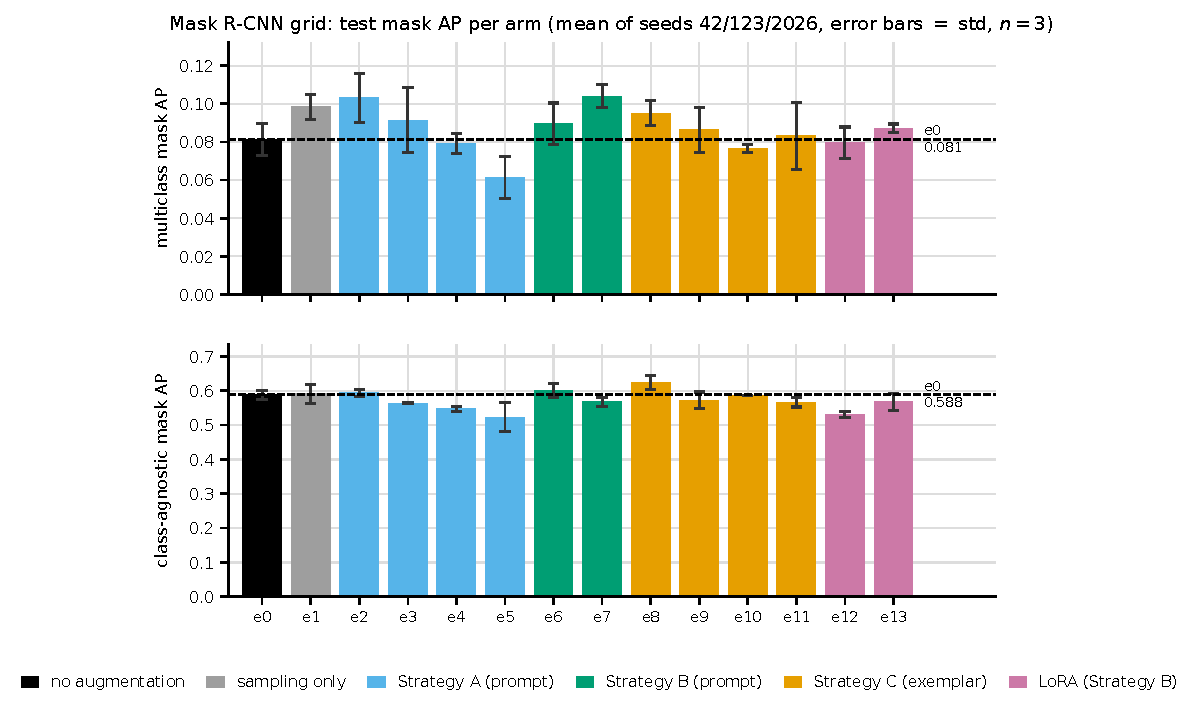
\includegraphics[width=\textwidth]{images/fig_grid_ap.pdf}
\caption{Mask R-CNN grid: mask AP per arm in both tracks.}
\label{fig:gridap}
\end{figure}

The class-agnostic track is the more legible half of the grid, because its
standard deviations are proportionally much smaller. The baseline is
$0.588 \pm 0.013$. The best arm is copy-paste at $0.624 \pm 0.020$, a difference
of $+0.036$ with all three seeds positive; the worst is the LoRA conversion at
$0.531 \pm 0.010$, a difference of $-0.057$ with all three seeds negative. Nine
of the thirteen augmented arms fall below the baseline: e3, e4, e5, e7, e9, e10,
e11, e12 and e13. Only e1, e2, e6 and e8 are above it. Every paired sign test
again returns $p \ge 0.25$, so none of these differences --- including the
$+0.036$ of copy-paste and the $-0.057$ of LoRA --- meets a conventional
significance threshold at this sample size. What the pattern does support is a
directional statement that does not depend on any single test: the arms that add
diffusion-generated pixels (e2--e5, e10--e13) are distributed around and mostly
below the baseline, and the one arm that adds only real transplanted pixels is
the highest.

Rare-class macro AP, the quantity the entire augmentation effort was designed to
raise, is effectively zero everywhere. The largest value in the grid is $0.0036$
for copy-paste, and its three seeds are $\{0.0108, 0.0000, 0.0000\}$ --- a single
seed in which one rare instance happened to be matched. The paired test on this
metric returns $p = 1.00$. Six of the fourteen arms score exactly $0.0000$.
Figure~\ref{fig:raremacro} plots these values on an axis scaled to the
class-agnostic baseline, which is the clearest single statement of the project's
outcome: the bars are invisible.

\begin{figure}[H]
\centering
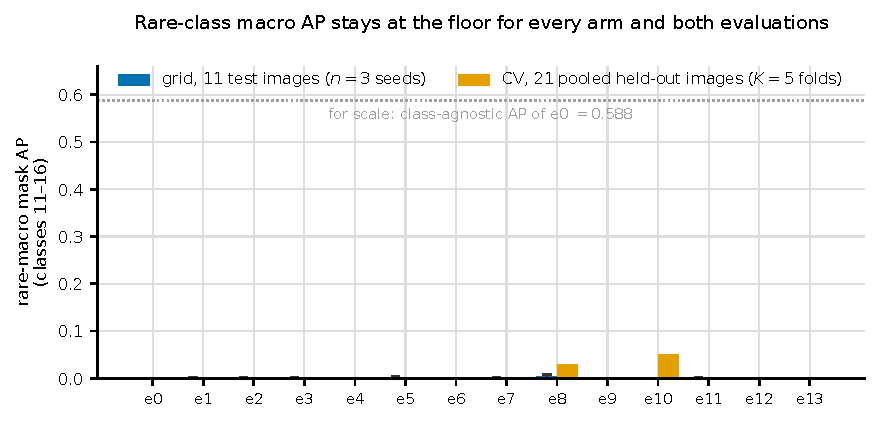
\includegraphics[width=\textwidth]{images/fig_rare_macro.pdf}
\caption{Rare-class macro AP across arms and both evaluations.}
\label{fig:raremacro}
\end{figure}

\subsection*{Experiment 2: rotated held-out cross-validation}

The grid's test split is 11 images. The cross-validation re-evaluates the frozen
grid checkpoints on five disjoint folds of the 21 held-out images, so every
held-out image is scored exactly once and the pooled rare support rises from 17
to 40 instances. Results for the six selected arms are in Table~\ref{tab:cv}.

\begin{table}[H]
\centering
\caption{Rotated held-out cross-validation, $K=5$ folds over 21 held-out images,
evaluation-only on the frozen grid checkpoints. Mean $\pm$ std over folds;
``pos.\ folds'' counts folds in which the arm exceeded e0; $p$ is the exact
two-sided paired sign test over folds, whose minimum attainable value at $K=5$ is
$0.0625$. Source: \protect\path{outputs/final/cv/summary.csv} and \texttt{summary.json}.}
\label{tab:cv}
\small
\begin{tabular}{@{}ll rrrr r rrr@{}}
\toprule
& & \multicolumn{4}{c}{Multiclass overall AP} & rare & \multicolumn{3}{c}{Class-agnostic overall AP} \\
\cmidrule(lr){3-6}\cmidrule(lr){7-7}\cmidrule(lr){8-10}
Arm & Method & AP & $\Delta$ & pos. & $p$ & macro AP & AP & $\Delta$ & pos. \\
\midrule
e0  & Original            & $0.143 \pm 0.037$ & ---      & ---  & ---   & $0.000$ & $0.602 \pm 0.044$ & ---      & --- \\
e1  & Rare-weighted       & $0.154 \pm 0.019$ & $+0.011$ & 3/5  & 1.000 & $0.000$ & $0.615 \pm 0.072$ & $+0.013$ & 3/5 \\
e6  & Strategy B          & $0.153 \pm 0.013$ & $+0.010$ & 2/5  & 1.000 & $0.000$ & $0.626 \pm 0.060$ & $+0.024$ & 4/5 \\
e8  & C copy-paste        & $0.152 \pm 0.020$ & $+0.010$ & 4/5  & 0.375 & $0.029$ & $\mathbf{0.647 \pm 0.061}$ & $+0.045$ & \textbf{5/5} \\
e10 & C diffusion inpaint & $0.135 \pm 0.032$ & $-0.008$ & 2/5  & 1.000 & $0.050$ & $0.616 \pm 0.061$ & $+0.014$ & 3/5 \\
e12 & LoRA Strategy B     & $0.134 \pm 0.020$ & $-0.008$ & 3/5  & 1.000 & $0.000$ & $0.568 \pm 0.077$ & $-0.034$ & 1/5 \\
\bottomrule
\end{tabular}
\end{table}

The multiclass picture is unchanged: the six arms span $0.134$ to $0.154$ against
a baseline of $0.143 \pm 0.037$, the two diffusion-based arms (e10, e12) are the
two lowest, and no paired test falls below $p = 0.375$. Overall AP is roughly
twice its grid value in every arm, which reflects the different composition of
the evaluation set rather than any change in the models --- the folds include the
former validation images, which are drawn from a project whose plans the
detectors find easier.

The class-agnostic column contains the one result in the project with a
consistent sign. Copy-paste scores $0.647 \pm 0.061$ against $0.602 \pm 0.044$,
a difference of $+0.045$ that is positive in all five folds
($\{+0.070, +0.033, +0.016, +0.040, +0.067\}$). The exact two-sided sign test
gives $p = 0.0625$, which is the smallest value obtainable with $K = 5$ and
therefore does not clear $0.05$ no matter how consistent the effect is. This is a
limit of the design, not of the result, and it is stated as such: five folds
cannot produce a conventionally significant two-sided sign test. The remaining
class-agnostic arms are further from significance still: $p = 1.000$ for e1 and
e10, $p = 0.375$ for e6 and for e12's negative $-0.034$. The honest summary is
that copy-paste shows a small positive effect that replicated across every fold
and across both Mask R-CNN evaluations, and that the evidence is suggestive
rather than conclusive. Figure~\ref{fig:cvagnostic} shows the fold
structure directly.

\begin{figure}[H]
\centering
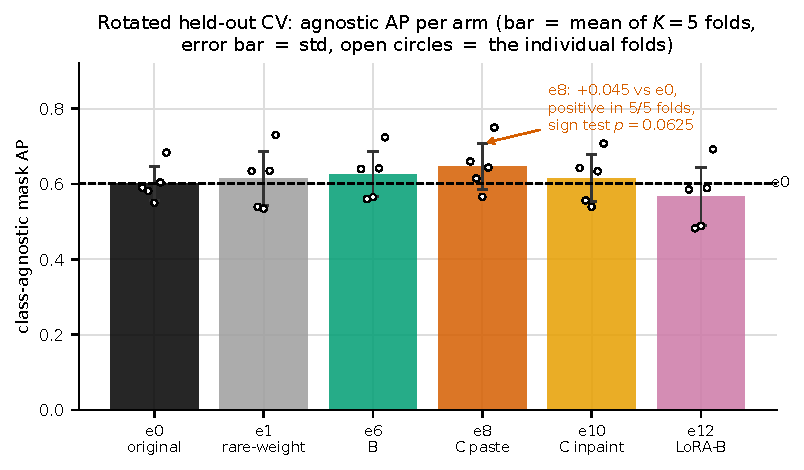
\includegraphics[width=\textwidth]{images/fig_cv_agnostic.pdf}
\caption{Cross-validation: class-agnostic AP per arm with per-fold points.}
\label{fig:cvagnostic}
\end{figure}

Pooling the folds also gives the first non-zero rare numbers in the project, and
they are worth stating precisely because they look better than they are. The
pooled rare-macro AP is $0.050$ for e10 and $0.029$ for e8, against $0.000$ for
e0, e1, e6 and e12. In both cases the entire value comes from a single category:
Abstellraum (class 12, pooled support 3 instances), which reaches a pooled mask
AP of $0.300$ for e10 and $0.176$ for e8. The other five primary-rare categories
score exactly $0.000$ in every arm, including Allg.\ Verkehrsfl\"ache with the
largest pooled rare support of 13 instances. A rare-macro AP of $0.05$ driven by
three instances of one class is not evidence that inpainting augmentation
improves rare-class segmentation.

\subsection*{Experiment 3: SAM 3}

Table~\ref{tab:sam3} gives the SAM 3 runs alongside the matched Mask R-CNN arms,
and Figure~\ref{fig:sam3} plots the comparison. Each SAM 3 cell is a single
training run; the Mask R-CNN cells are means over three seeds with their standard
deviations, which is what makes the comparison interpretable.

\begin{table}[H]
\centering
\caption{SAM 3 versus Mask R-CNN on the same test split and the same augmented
datasets. SAM 3 values are single runs ($n=1$, no std available); Mask R-CNN
values are mean $\pm$ std over three seeds. Sources:
\protect\path{outputs/final/sam3/summary.csv} and
\protect\path{outputs/final/grid_r1/summary.csv}.}
\label{tab:sam3}
\small
\begin{tabular}{@{}ll rr rr@{}}
\toprule
& & \multicolumn{2}{c}{Multiclass mask AP} & \multicolumn{2}{c}{Class-agnostic mask AP} \\
\cmidrule(lr){3-4}\cmidrule(lr){5-6}
Training data & Arm & SAM 3 ($n{=}1$) & Mask R-CNN ($n{=}3$) & SAM 3 ($n{=}1$) & Mask R-CNN ($n{=}3$) \\
\midrule
Original (no aug)    & e0  & $0.115$ & $0.081 \pm 0.008$ & $\mathbf{0.713}$ & $0.588 \pm 0.013$ \\
C diffusion inpaint  & e10 & $0.120$ & $0.077 \pm 0.002$ & $0.704$ & $0.586 \pm 0.001$ \\
LoRA Strategy B      & e12 & $0.140$ & $0.080 \pm 0.008$ & $0.685$ & $0.531 \pm 0.010$ \\
C copy-paste         & e8  & $\mathbf{0.147}$ & $0.095 \pm 0.007$ & $0.693$ & $0.624 \pm 0.020$ \\
\midrule
\multicolumn{2}{@{}l}{$\Delta$ vs.\ own baseline, best aug.} & $+0.032$ & $+0.014$ & $-0.009$ & $+0.036$ \\
\bottomrule
\end{tabular}
\end{table}

\begin{figure}[H]
\centering
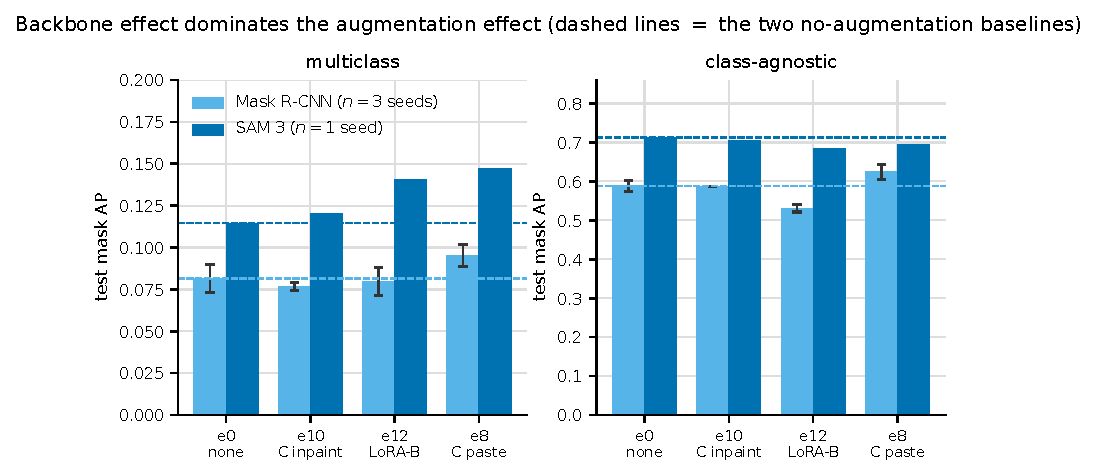
\includegraphics[width=\textwidth]{images/fig_sam3_vs_mrcnn.pdf}
\caption{SAM 3 against Mask R-CNN, baseline and augmented, in both tracks.}
\label{fig:sam3}
\end{figure}

On the multiclass track SAM 3 improved under all three augmentations: $+0.005$
for diffusion inpaint, $+0.026$ for the LoRA conversion and $+0.032$ for
copy-paste, the last being the largest positive augmentation effect measured
anywhere in the project. It is nevertheless not evidence of an effect. Each value
is a single run, and the seed-to-seed standard deviation measured on the Mask
R-CNN multiclass grid ranges from $0.002$ to $0.018$, with individual arms
spanning up to $0.031$ across their three seeds. All three SAM 3 deltas lie
inside that band, so a plausible alternative explanation is that they are the
draw of one seed. Reporting them as improvements would require the three-seed
repetition that queue time did not allow.

On the class-agnostic track the direction reverses: every augmentation lowered
SAM 3's AP, from $0.713$ at baseline to $0.704$, $0.693$ and $0.685$. The sign
of the copy-paste effect is therefore opposite in the two backbones ($+0.036$ for
Mask R-CNN, $-0.020$ for SAM 3), which is itself an argument against reading any
of these single-run deltas as a property of the augmentation.

The one comparison in Table~\ref{tab:sam3} that is not fragile is the vertical
one. SAM 3's unaugmented class-agnostic AP of $0.713$ exceeds the best Mask R-CNN
arm ($0.624$ for e8) by $0.089$, and its unaugmented multiclass AP of $0.115$
exceeds the best Mask R-CNN arm ($0.104$ for e7) by $0.011$. The class-agnostic
gap is roughly two and a half times the largest augmentation delta measured in
the entire grid and an order of magnitude above the typical one. Whatever benefit
augmentation might carry at this data scale, backbone choice dominates it.

\subsection*{Experiment 4: the two-stage DINOv2 pipeline}

Stage 2 was trained on 887 real training crops, optionally extended with the 171
synthetic rare crops produced by the augmentation pipeline, and evaluated both on
368 real ground-truth test crops (Evaluation A) and end-to-end over 483
class-agnostic SAM 3 test proposals (Evaluation B). Table~\ref{tab:dino} gives
both.

\begin{table}[H]
\centering
\caption{Two-stage room typing with a frozen DINOv2-base encoder.
Evaluation A classifies 368 ground-truth test crops, removing detector error;
Evaluation B labels 483 class-agnostic SAM 3 proposals and scores the result as
multiclass instance segmentation on the same test split as every other
experiment. Single runs. Source: \protect\path{outputs/final/dino/summary.csv} and
\texttt{report.md}.}
\label{tab:dino}
\small
\begin{tabular}{@{}ll rrr rr@{}}
\toprule
& & \multicolumn{3}{c}{Evaluation A: GT-crop classification} & \multicolumn{2}{c}{Evaluation B: two-stage} \\
\cmidrule(lr){3-5}\cmidrule(lr){6-7}
Head training set & Head & top-1 & head-macro rec. & rare-macro rec. & mask AP & rare AP \\
\midrule
real (887 crops)          & linear & $\mathbf{0.454}$ & $\mathbf{0.381}$ & $0.000$ & $\mathbf{0.0910}$ & $0.0000$ \\
real (887 crops)          & kNN    & $0.386$ & $0.332$ & $0.000$ & $0.0797$ & $0.0000$ \\
real $+$ 171 synth.\ rare & linear & $0.440$ & $0.354$ & $0.000$ & $0.0892$ & $0.0000$ \\
real $+$ 171 synth.\ rare & kNN    & $0.340$ & $0.286$ & $0.000$ & $0.0748$ & $0.0042$ \\
\midrule
\multicolumn{5}{@{}l}{\emph{reference, end-to-end fine-tuned, same test split:} SAM 3 multiclass} & $0.115$ & \\
\multicolumn{5}{@{}l}{\emph{reference:} best Mask R-CNN arm (e7, $n{=}3$)} & $0.104$ & \\
\multicolumn{5}{@{}l}{\emph{reference:} Mask R-CNN e0 ($n{=}3$)} & $0.081$ & \\
\bottomrule
\end{tabular}
\end{table}

Evaluation A is the diagnostic result of the project. Given perfect
ground-truth crops --- no detector error at all --- a frozen DINOv2-base encoder
with a linear head reaches $0.454$ top-1 over 19 classes and $0.381$ macro recall
over the ten head classes, but $0.000$ macro recall over the six primary-rare
classes. That zero holds in every arm and for both heads. Figure~\ref{fig:dinorecall}
shows the per-class breakdown: recall is $0.96$ for Treppe, $0.82$ for WC and
$0.69$ for Aufzug, then collapses --- $0.15$ for Lager, $0.08$ for Technikraum,
and exactly zero for K\"uche, ``Flur, Halle'', Besprechungsraum and all six rare
classes. Since localisation is not involved, this locates the failure squarely in
room-type classification, and it shows that the failure is not confined to the
tail: four head classes with 3--16 test instances also score zero.

\begin{figure}[H]
\centering
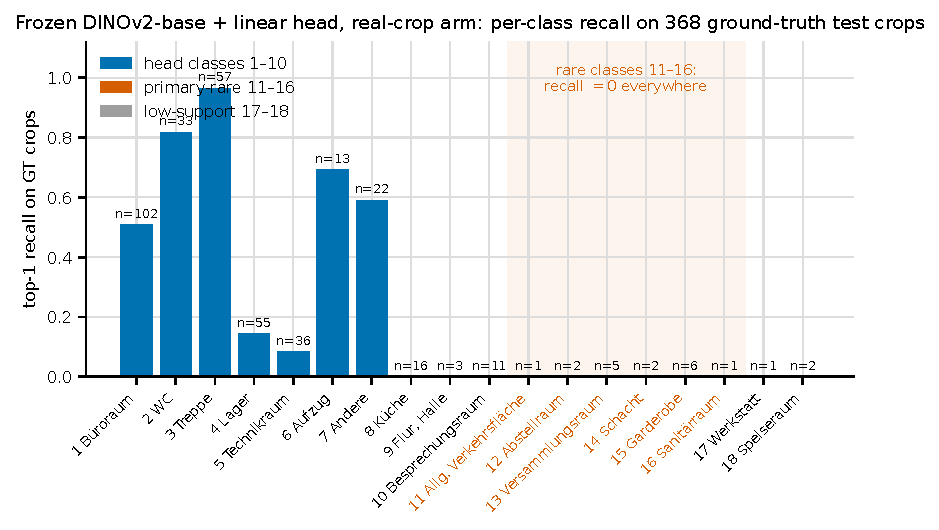
\includegraphics[width=\textwidth]{images/fig_dino_recall.pdf}
\caption{Per-class recall of the frozen DINOv2 classifier on ground-truth crops.}
\label{fig:dinorecall}
\end{figure}

Adding the 171 synthetic rare crops did not help. Top-1 accuracy fell from
$0.454$ to $0.440$ for the linear head and from $0.386$ to $0.340$ for kNN,
head-macro recall fell in both, and rare-macro recall stayed at $0.000$. The
synthetic crops were produced by the same pipeline whose output the detectors
also declined to benefit from, so the result is consistent rather than
surprising, but it closes off the hypothesis that the crops were useful data that
the detector setting simply failed to exploit. The single non-zero rare number in
the whole table --- a two-stage rare AP of $0.0042$ for the real-plus-synthetic
kNN arm --- comes from an arm whose overall accuracy is the worst of the four and
whose rare-macro recall is still zero.

Evaluation B places the pipeline on the same axis as the fine-tuned detectors.
Its best configuration reaches $0.0910$ two-stage mask AP, below fine-tuned SAM 3
($0.115$) and below the best Mask R-CNN arm ($0.104$), and above only the
unaugmented Mask R-CNN baseline ($0.081$). Figure~\ref{fig:dinotwostage} shows
this against the three reference lines. Decomposing the problem therefore did not
recover the accuracy that end-to-end fine-tuning achieves, even though stage 1 is
the strongest localiser available: SAM 3 finds room boundaries at $0.713$
class-agnostic AP, and the two-stage system converts that into $0.091$ multiclass
AP. The gap between those two numbers is the classification problem, measured
end-to-end.

\begin{figure}[H]
\centering
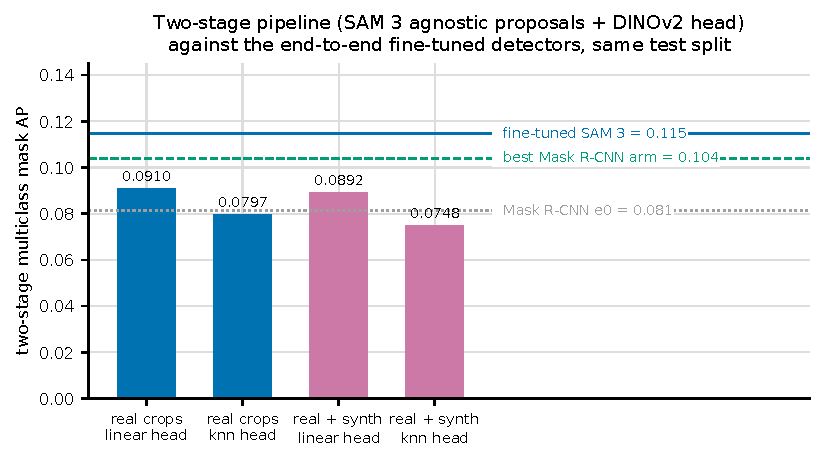
\includegraphics[width=\textwidth]{images/fig_dino_twostage.pdf}
\caption{Two-stage mask AP against the end-to-end fine-tuned detectors.}
\label{fig:dinotwostage}
\end{figure}

\subsection*{Qualitative check}

Figure~\ref{fig:predmulticlass} pairs ground truth with the multiclass Mask R-CNN
prediction on test plan 034, and Figure~\ref{fig:predagnostic} does the same for
the class-agnostic model. The contrast is the numerical result made visible. The
class-agnostic model recovers nearly every room polygon in the plan, including
the small service rooms along the perimeter. The multiclass model on the same
image recovers the corridor network and the two Luftr\"aume, but leaves a large
share of the offices, the meeting rooms and the Abstellraum in the upper left
uncoloured, and predicts no rare-class instance anywhere on the plan. The two
panels differ only in the label space of the model that produced them. This is
the same story as
Tables~\ref{tab:grid}--\ref{tab:dino}: the geometry is available and the label is
not.

\begin{figure}[H]
\centering
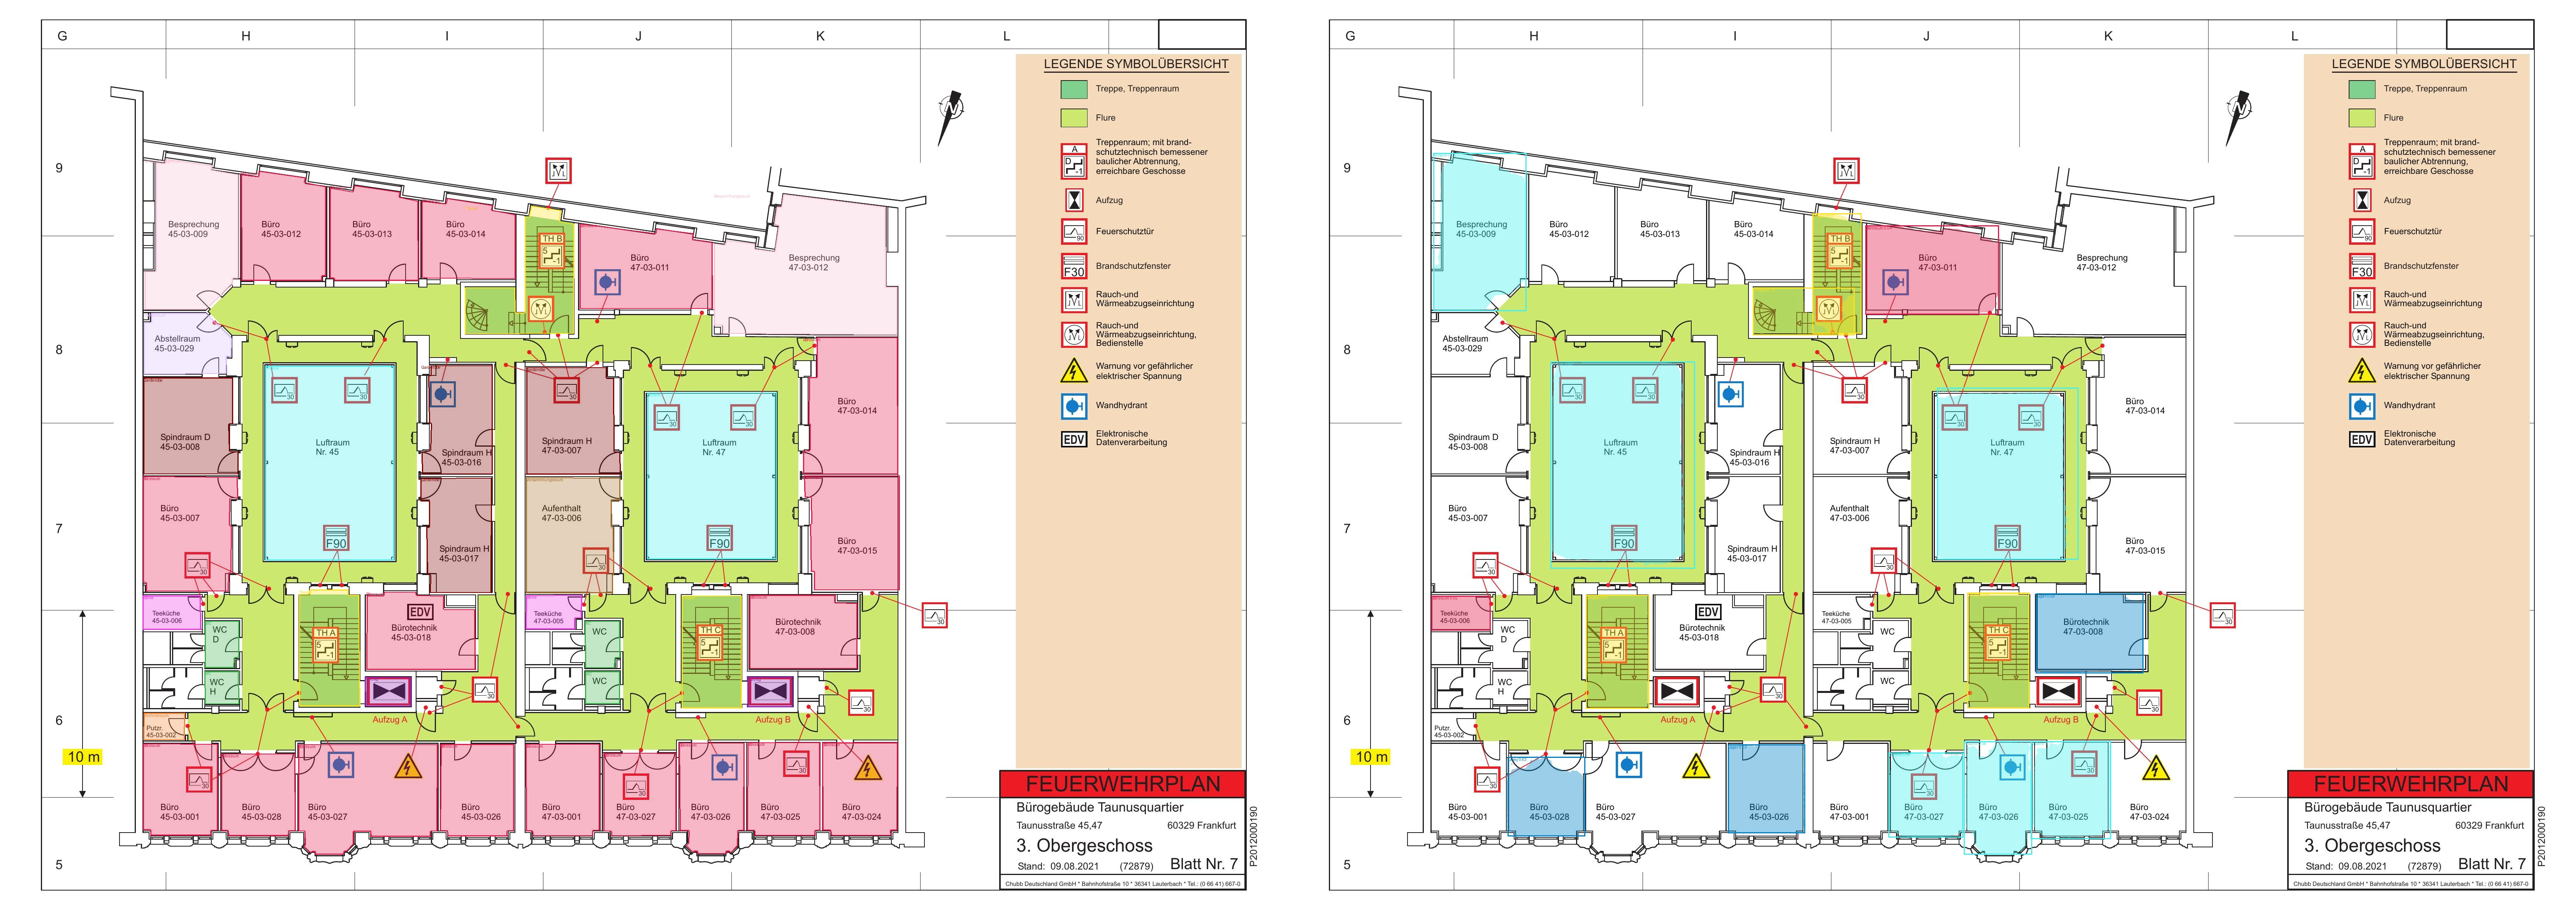
\includegraphics[width=\textwidth]{images/mrcnn_multiclass_034.jpg}
\caption{Multiclass Mask R-CNN: ground truth (left) versus prediction (right).}
\label{fig:predmulticlass}
\end{figure}

\begin{figure}[H]
\centering
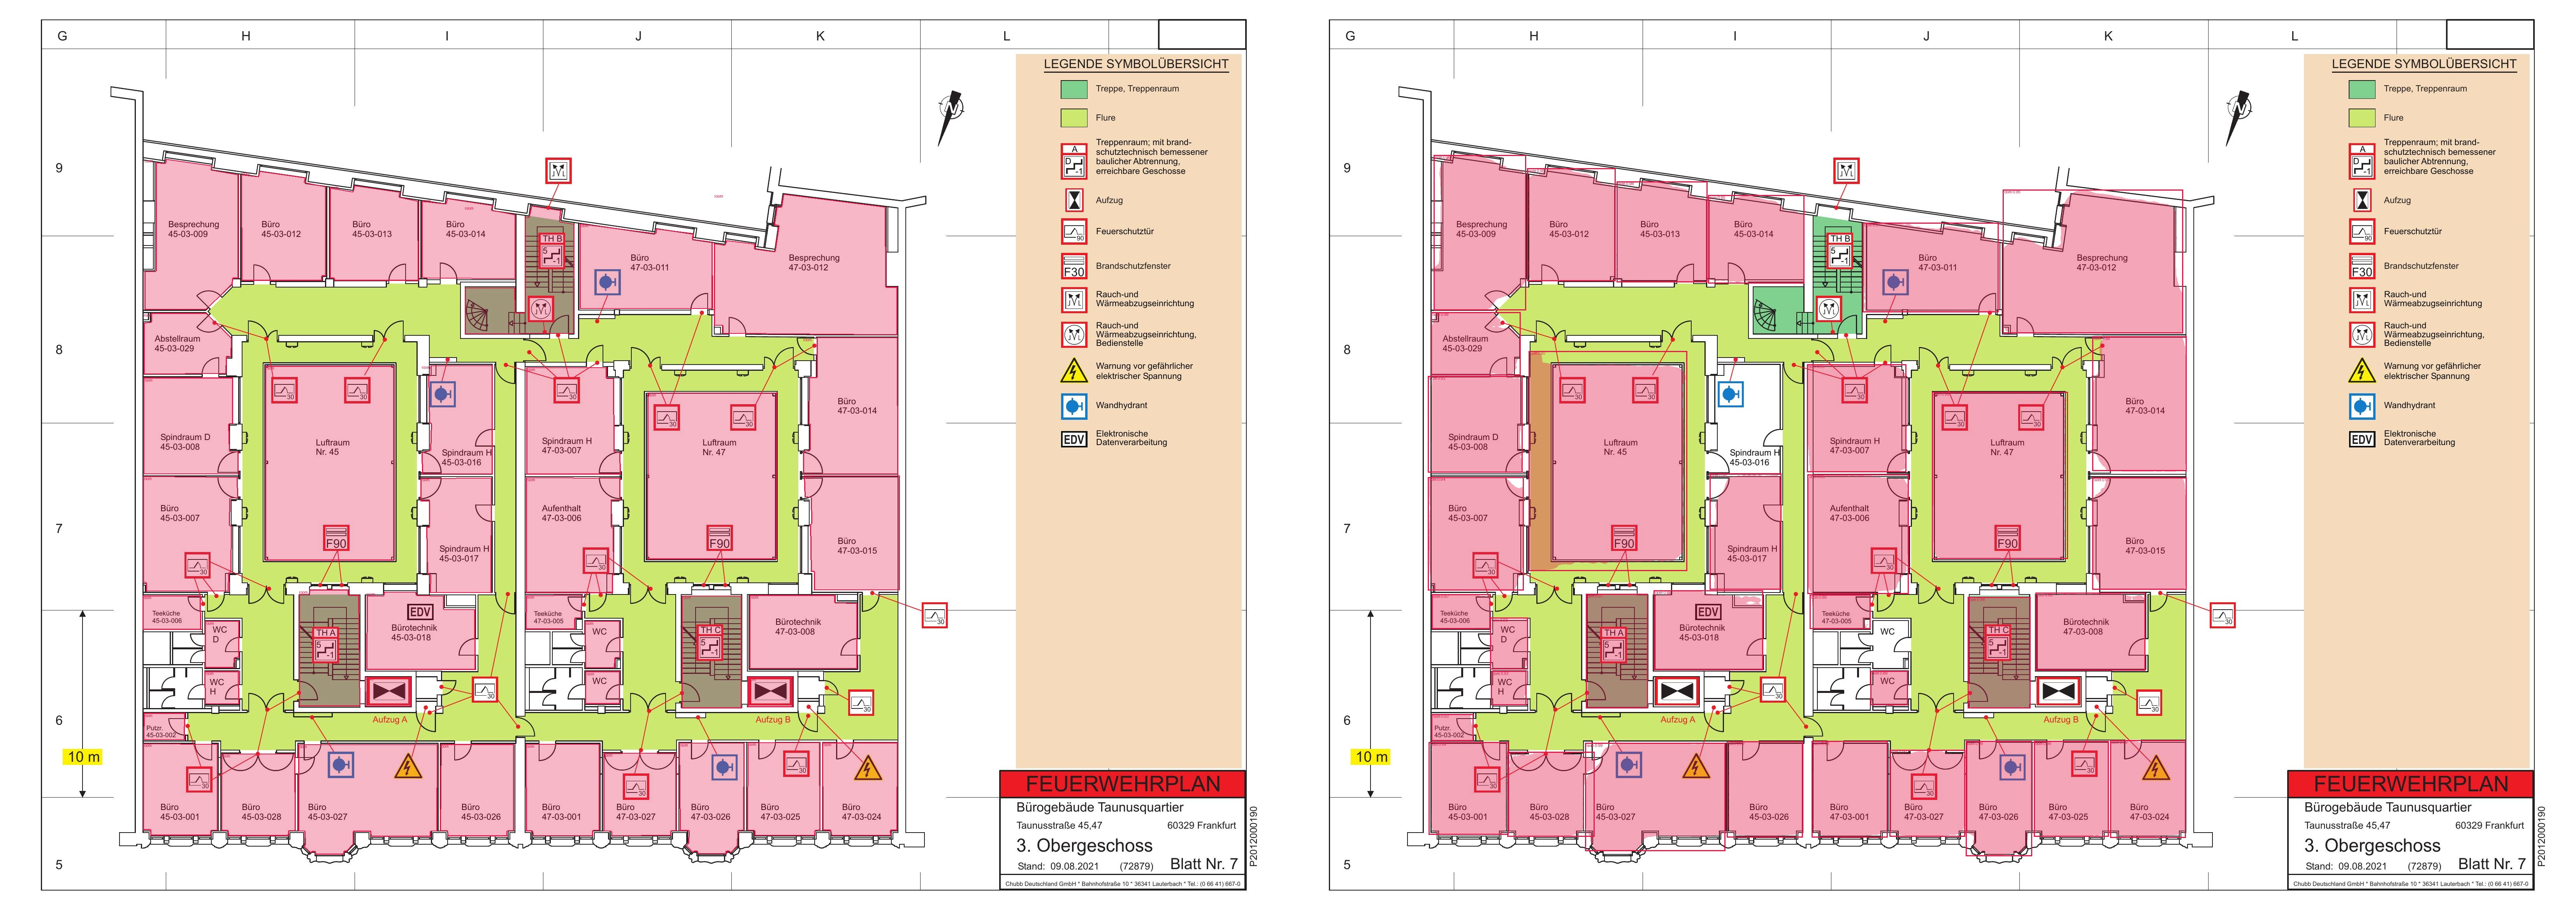
\includegraphics[width=\textwidth]{images/mrcnn_agnostic_034.jpg}
\caption{Class-agnostic Mask R-CNN on the same test plan.}
\label{fig:predagnostic}
\end{figure}

\subsection*{Summary of the evidence}

Reading the four experiments together, three statements are supported and one
frequently-made statement is not.

Diffusion and LoRA inpainting augmentation did not reliably improve floor-plan
room segmentation. On Mask R-CNN the effect is neutral to harmful and replicated
as such across three seeds and five cross-validation folds: nine of thirteen
augmented arms fall below baseline on the class-agnostic grid, the two
diffusion-based arms are the two lowest multiclass arms in the cross-validation,
and the LoRA arm is the worst arm in the grid at $-0.057$. On SAM 3 there is a
small multiclass gain that is unreplicated, single-seed, and inside the noise
band measured on the grid, accompanied by a class-agnostic loss under every
augmentation. As classifier-crop augmentation the synthetic data lowered every
metric it touched.

Simple exemplar copy-paste --- the control arm containing no generated pixels ---
is the only augmentation with a small, consistent positive effect. It is the
top-ranked arm in three of the six backbone $\times$ track comparisons run in the
project (Mask R-CNN class-agnostic grid, Mask R-CNN class-agnostic
cross-validation, SAM 3 multiclass); it is not top-ranked in the Mask R-CNN
multiclass grid (e7 leads), the multiclass cross-validation (e1 leads), or the
SAM 3 class-agnostic track (the baseline leads). Its strongest single result is
the cross-validated $+0.045$ class-agnostic AP, positive in all five folds at
$p = 0.0625$.

The backbone dominates the augmentation. SAM 3 exceeds the best Mask R-CNN arm by
$0.089$ class-agnostic AP and $0.011$ multiclass AP without any augmentation at
all, and the class-agnostic figure is larger than every augmentation delta
measured in the project.

What is not supported is the premise the project set out to test. Rare-class room
segmentation is not merely unimproved by augmentation; it is out of reach at this
data scale by any method tried. Rare AP is at or near zero across all fourteen
arms, both backbones and both evaluation protocols, and rare-macro recall is
exactly zero even when a frozen classifier is handed perfect ground-truth crops.
With 17 rare test instances --- 40 when pooled over the cross-validation --- the
experiment can exclude a large effect and cannot resolve a small one. Meanwhile
class-agnostic localisation already works, at $0.588$--$0.647$ AP for Mask R-CNN
and $0.713$ for SAM 3. The unsolved component is room-type classification, and a
dedicated frozen classifier did not fix it.


\section{Conclusions and Future Scope}

The project set out to determine whether diffusion or LoRA inpainting of rare
room types improves room-instance segmentation of architectural floor plans, and
whether that answer depends on the backbone. The measured answer is that it does
not improve segmentation, and that the backbone matters far more than the
augmentation.

Goal 1 was achieved as specified. Fourteen controlled arms were built on
leakage-safe generators that read only frozen training identifiers, each accepted
sample passing automated geometry, pixel-quality and exact-structural-invariance
checks with a recorded decision audit and output hash, and each arm training
under the identical model, schedule and 35-step-per-epoch budget in both the
multiclass and class-agnostic views. The matrix included the non-generative
controls that make the diffusion treatment interpretable, and it was that design
choice --- rather than any positive finding --- that produced the project's most
useful result.

Goal 2 was achieved in the sense the goal statement anticipated: a defensible
answer was obtained, and the answer is a null result. Across 84 Mask R-CNN
training runs, no augmentation arm produced a difference from the unaugmented
baseline that the data supports. Every paired sign test on the three-seed grid
returned $p \ge 0.25$, and $0.25$ is the floor of the test at $n=3$. Nine of the
thirteen augmented arms scored below baseline on the class-agnostic track, the
LoRA conversion worst at $-0.057$. The cross-validation over 21 held-out images
reproduced the same ordering. The single result with a consistent sign is
exemplar copy-paste at $+0.045$ class-agnostic AP, positive in all five folds at
$p = 0.0625$ --- and copy-paste is the control arm that contains no generated
pixels, which is the opposite of the hypothesis under test. It is also the
outcome Ghiasi et al.\ \cite{ghiasi2021copypaste} would have predicted.

Goal 3 changed the framing of the project. SAM 3 without any augmentation
reached $0.713$ class-agnostic and $0.115$ multiclass mask AP, exceeding the best
Mask R-CNN arm by $0.089$ and $0.011$ respectively. The class-agnostic gap is
about two and a half times the largest augmentation delta measured anywhere in
the grid. Under augmentation SAM 3 showed a $+0.032$ multiclass gain from
copy-paste, but on a single seed, inside the $0.002$--$0.018$ seed-noise band
measured on the grid, and accompanied by a class-agnostic loss under all three
augmentations --- so the sign of the copy-paste effect is opposite in the two
backbones. That inconsistency is itself the finding: at this data scale the
augmentation effect is not a stable property of the augmentation.

Goal 4 supplied the diagnosis. Handing a frozen DINOv2-base encoder perfect
ground-truth crops --- no detector error whatsoever --- yielded $0.454$ top-1
accuracy over 19 classes and exactly $0.000$ macro recall over the six
primary-rare classes, in every arm and for both heads. Adding the 171 synthetic
rare crops lowered top-1 accuracy in both heads and left rare recall at zero. The
end-to-end two-stage system reached $0.091$ mask AP, below both fine-tuned
detectors. Combined with the class-agnostic results, this locates the failure
precisely: room \emph{localisation} is largely solved on this dataset at
$0.59$--$0.71$ AP, and room \emph{typing} is not, for the tail or for several head
classes either. No augmentation of the training pixels was going to fix a
classification problem of that shape.

The wider conclusion is a scope statement rather than a defeat. The generative
augmentation literature surveyed in Section~3 reports its gains on benchmarks
with 100k training images where a ``rare'' class still has a few hundred
instances \cite{gupta2019lvis,xie2024mosaicfusion,shin2023fillup}. This project
had 35 training plans, 30 rare training instances and 17 rare test instances. In
that regime the measurement itself is the binding constraint: an AP computed over
one or two instances is a step function, and the experiment can exclude a large
rare-class effect but cannot resolve a small one. The qualitative evidence in
Figures~\ref{fig:qastrategya} and \ref{fig:loraval} suggests the mechanism as
well. A pretrained diffusion model asked to draw a German Versammlungsraum
produces perspective furniture, and the LoRA adapter that fixed the domain
mismatch learned mostly that floor plans are white space --- partly because the
mask construction protects detected dark strokes, and the printed room labels and
symbols that identify a room type are exactly those strokes. The safety
machinery that made the augmentation trustworthy also removed most of what
carried the class signal.

\subsection*{Future scope}

Four directions follow from the measurements rather than from speculation, and
they are ordered by expected value per unit of effort.

\emph{Read the drawing's own text.} Every plan in this dataset prints the room
type inside the room --- ``B\"uro'', ``Technik'', ``Abstellraum''. The vision-only
classifier scored zero recall on all six rare classes while that label sat inside
the crop it was given. Pairing the class-agnostic detector, which already works,
with OCR or a vision-language model over the crop is the obvious next experiment,
and WAFFLE \cite{ganon2025waffle} demonstrates the approach at scale on
heterogeneous floor plans. This is likely to move the multiclass number more than
anything attempted in this project.

\emph{Try a loss-side long-tail treatment before any further data synthesis.} The
project spent its effort on the data and none on the objective. A Seesaw loss
\cite{wang2021seesaw} costs one configuration change, needs no generator, and
attacks the classification imbalance the two-stage experiment identified as the
actual failure. It should be run on the SAM 3 backbone, which is where the
headroom is.

\emph{Fix the semantic gap in generation, or steer instead of adapting.} If
generative augmentation is revisited, the two concrete fixes are already
identified in the literature. Gen-n-Val \cite{huang2025gennval} shows that a
semantic validator, not more generation, is the binding constraint --- our
pipeline could certify structural safety but recorded
\texttt{semantic\_correctness = unverified} for every prompt-based sample. DoGE
\cite{wang2024doge} avoids adapter training entirely by steering a frozen
generator with a domain-gap embedding, which suits a 30-instance tail better than
LoRA fine-tuning does. The revised ``semantic v2'' generator implemented late in
this project --- masking compact interior labels while preserving structural
lines, and seeding generation with a real rare exemplar --- is built but was not
run through the full grid, and it is the cheapest of these to complete. TMI
\cite{song2026tmi} additionally predicts that the prompt-driven and
exemplar-driven families are complementary and that neither works alone, which
matches what was observed here and suggests the combination is worth one run.

\emph{Collect more rare-class test data before running anything else.} This is
the least interesting recommendation and the most important one. Seventeen rare
test instances cannot support the claim the project was designed to make, and no
amount of methodological care removes that ceiling. Roughly a hundred rare test
instances --- reachable by annotating a few dozen further plans from the same
archive --- would make the difference between excluding a large effect and
measuring a real one. Until that exists, the defensible use of this dataset is
class-agnostic room extraction, where both backbones already perform well, with
room typing handled by the printed labels rather than by appearance.


\medskip

\bibliographystyle{unsrt}
\bibliography{references}

\end{document}
